
\documentclass[letterpaper,twoside,12pt]{report}

%%%%%%%%%%%%% Language %%%%%%%%%%%%%%%%%%%%%%%%%%%%%%%%%%%%%%%%%%%%%%%%%%%%%%%%%%%%%%%%%%
%\usepackage{colortbl} %creates fill colours etc in tables
\usepackage[USenglish]{babel} %francais, polish, spanish, ...
\usepackage[T1]{fontenc}
\usepackage[ansinew]{inputenc}
\usepackage{lmodern} %Type1-font for non-english texts and characters
\usepackage{multirow}
\usepackage{graphicx} %%For loading graphic files
\usepackage{float} %allows graphics to be positioned accurately
\usepackage{longtable}

%%%%%%%%%%%%%Page setup%%%%%%%%%%%%%%%%%%%%%%%%%%%%%%%%%%%%%%%%%%%%%%%%%%%%%%%%%%%%%%%%%%
\oddsidemargin 0in
\evensidemargin 0in
\textwidth 6.5in
\headheight 0.0in
\topmargin -0.75in
\textheight 8.75in

\usepackage{color}
\usepackage{array}
\usepackage{colortbl}
\usepackage{fancyhdr}
\fancyhead{}
\renewcommand{\headheight}{0.6in}
\fancyhead[R]{
\includegraphics[height=.4in]{OptimumT_Logo_full_text.png}}

%footer definition
\fancyfoot{}
\fancyfoot[C]{\thepage}  
\fancyfoot[R]{Optimum T \\ Help File} 
\pagestyle{fancyplain}

%Paragraph settings
\setlength{\parindent}{0pt} 
\setlength{\parskip}{1.5ex}

%% Math Packages %%%%%%%%%%%%%%%%%%%%%%%%%%%%%%%%%%%%%%%%%%%%%%%%%%%%%%%%%%%%%%%%%%%%%%%%
\usepackage{amsmath}
\usepackage{amsthm}
\usepackage{amsfonts}

\usepackage[pdftex,pdfpagelabels,hypertexnames=true,plainpages=false,naturalnames, bookmarks=true, bookmarksnumbered=true, breaklinks=true, linkbordercolor={1 1 1}]{hyperref} %\usepackage[,pagebackref,]{hyperref}
%\usepackage[pdftex, bookmarks=true, bookmarksnumbered=true, breaklinks=true, linkbordercolor={1 1 1}]{hyperref}
\usepackage[all]{hypcap}

%define colors to be used for section headings and table background fills
\definecolor{bblue}{rgb}{0.2,0.3,0.5}
\definecolor{tblue}{rgb}{0.392, 0.584, 0.929}
\definecolor{ttblue}{rgb}{0.795, 0.88, 1}

%Redefine the subsection definition
%\makeatletter
%\renewcommand{\subsection}{\@startsection
%{subsection}
%{3}
%{0mm}
%{-3.5ex \@plus -1ex \@minus -.2ex}
%{2.3ex \@plus.2ex}
%{\normalfont\large\bfseries\textcolor{bblue}}}
%\makeatother

%Redefine the section definition to include a page break before each new section
%\makeatletter
%\renewcommand{\section}{\@startsection
%{section}
%{2}
%{0mm}
%{-3.5ex \@plus -1ex \@minus -.2ex}
%{2.3ex \@plus.2ex}
%{\normalfont\Large\bfseries\textcolor{bblue}}}
%\makeatother

%redefine the chapeter heading to remove the word "chapter"
%\makeatletter
%\renewcommand{\@makechapterhead}[1]{%
%\vspace*{0 pt}
%{\setlength{\parindent}{0pt} \raggedright \normalfont
%\Huge \bfseries \textcolor{bblue}{ \thechapter.\ #1}
%\par\nobreak\vspace{30 pt}}}
%\makeatother

%put dot spacing in contents page
%\makeatletter
%\renewcommand\l@chapter[2]{%
%  \ifnum \c@tocdepth >\z@
%    \addpenalty\@secpenalty
%    \addvspace{1.0em \@plus\p@}%
%    \setlength\@tempdima{1.5em}%
%    \begingroup
%      \parindent \z@ \rightskip \@pnumwidth
%      \parfillskip -\@pnumwidth
%      \leavevmode \bfseries
%      \advance\leftskip\@tempdima
%      \hskip -\leftskip
%      #1\nobreak\ 
%      \leaders\hbox{$\m@th\mkern \@dotsep mu\hbox{.}\mkern \@dotsep mu$}
%     \hfil \nobreak\hb@xt@\@pnumwidth{\hss #2}\par
%    \endgroup
%  \fi}
%\makeatother

% Use the chapter number for the figures and tables
%\renewcommand{\thefigure}{\thesection.\arabic{figure}}
%\renewcommand{\thetable}{\thesection.\arabic{table}}

%insert an white space at the bottom of the page
\raggedbottom 
%%%%%%%%%%%%%%%%%%%%%%%%%%%%%%%%%%%%%%%%%%%%%%%%%%%%%%%%%%%%%%%%%%%%%%%%%%%%%%%%%%%%%%%%%%%%%%%%%%%%%%%%%
%%%%%%%%%%%%%%%%%%%%%%%%%%%%%%%%%%%%%%%%%%%%%%%%%%%%%%%%%%%%%%%%%%%%%%%%%%%%%%%%%%%%%%%%%%%%%%%%%%%%%%%%%

\begin{document}


\begin{titlepage}
\definecolor{darkblue}{RGB}{0,0,64}


\includegraphics[width=0.9\textwidth]{OptimumT_Logo_full_text.png}
\ \\
\vspace{0.8 in}
\begin{center}
\Huge{\textcolor{darkblue}{\textbf{Help File \\ Version 1.1}}}
\ \\
\vspace{1.6 in}
\large By \\

\includegraphics[width=0.7\textwidth]{OptimumGlogo.png}
~\href{mailto: engineering@optimumg.com}{engineering@optimumg.com}\\
~\href{http://www.optimumg.com}{www.optimumg.com}\\
\end{center}
\end{titlepage}



\chapter*{Welcome}
\label{sec:Welcome}
\addcontentsline{toc}{chapter}{Welcome}


Thank you for purchasing OptimumTire the new benchmark in tire model fitting and analysis. This help file contains information about all the functions and features of OptimumTire. Included in this help file are:
\begin{itemize}
	\item Information on how to use OptimumTire 
	\item Special Features in OptimumTire
	\item Tips and tricks on how to use OptimumTire efficiently
\end{itemize}
\section*{Feedback}
\label{sec:Feedback}
OptimumTire is a continually developing program and we give high regard to any suggestions, comments, complaints or criticisms that OptimumTire users might have. Please contact us at~\href{mailto: engineering@optimumg.com}{engineering@optimumg.com} and we will work to improve OptimumTire based on your feedback.

\section*{Features Coming Soon}
\label{sec:FeaturesComingSoon}

The following is a list of features that will be available in future updates. Please contact us if you have any suggestions on other features that should be included in OptimumTire in the future.
\begin{itemize}
	\item Additional Tire Models
	\item Automated Reports
	\item	Tire testing replay with model overlay
	\item	Temperature and time variables for analysis and creation of transient tire models
\end{itemize}


\tableofcontents


\chapter*{Introduction}
\addcontentsline{toc}{chapter}{Introduction}
\label{sec:Introduction}

Through OptimumG's consulting and seminar services, it identified tire data analysis and model fitting as an important, but often neglected area of vehicle dynamics. Therefore, OptimumTire was created from OptimumG's extensive knowledge and experience in testing, analysis, and development of vehicle tires and suspension systems. OptimumTire is a convenient and intuitive software package that allows users to perform advanced tire data analysis, visualization, and model fitting. 

Pacejka '96, 2002, and 2006 as well as MF5.2 and MF6.1 tire models are available in OptimumTire. Simpler Brush, Fiala and Harty models are also included. The models can be manually inputted, imported, or fit to raw tire data. The model fitting procedure is very fast and efficient partially due to the data processing tools incorporated into the software. All aspects of the tire models can be easily compared to the raw tire data to ensure accuracy. OptimumTire also allows adjustment of the tire models if necessary and includes scaling factors for the Pacejka models. These features ensure that the tire models created will accurately correlate to data collected from the road or race track. These tire models, as well as the processed data, can be exported from OptimumTire to a variety of file formats.

OptimumTire is also a very powerful data visualization tool.  It has the capability to display tire models and raw tire data in a user friendly but extremely powerful graphing utility. It features 2D and 3D graphing of over 30 different tire parameters. The ability to create surface plots and crossed line graphs allows the user to be able to easily create sophisticated graphs, like tire friction ellipses. The graphs can be further enhanced by including the effect of many different parameters including vertical load, inclination angle, and inflation pressure. These graphs can be easily copied or directly printed from the OptimumTire interface to be included in other projects or reports. The data from these graphs can also be exported for further analysis.
\chapter*{Installation Requirements}
\addcontentsline{toc}{chapter}{Installation Requirements}
\label{sec:InstallationRequirements}

\section*{Hardware Requirements}
\label{sec:HardwareRequirements}

\subsection*{Processor}
\label{sec:Processor}

\begin{itemize}
\item	Intel� Pentium 4�, Intel� Xeon�, and Intel� Core�  
\item	AMD� Athlon�, AMD� Opteron�, and AMD� Turion� 
\end{itemize}

\subsection*{Memory}
\label{sec:Memory}

\begin{itemize}
\item	Minimum: 512MB RAM
\item	Recommended: 1GB RAM or more
\item	Virtual Memory recommended to be twice the amount of RAM 
\end{itemize}

\subsection*{Storage}
\label{sec:Storage}

\begin{itemize}
\item Free space of at least 100MB. Includes installation of OptimumTire� and required software components (see below)
\end{itemize}

\subsection*{Display Adapter}
\label{sec:DisplayAdapter}

\begin{itemize}
\item	Minimum: Microsoft� DirectX� 9.0c capable graphics card with 32MB RAM
\item	Recommended: DirectX� 9.0c capable NVIDIA� GeForce� or ATI� Radeon� with 128MB RAM or higher
\end{itemize}

\subsection*{Display Unit}
\label{sec:DisplayUnit}

\begin{itemize}
\item	Minimum: 15" Screen with resolution of 1024 x 768 pixels
\item	Recommended: 19" Screen with resolution of 1280 x 1024 pixels
\end{itemize}

\subsection*{Other}
\label{sec:Other}

\begin{itemize}
\item	Mouse or other pointing device
\end{itemize}

\section*{Software Requirements}
\label{sec:SoftwareRequirements}

\subsection*{Operating System}
\label{sec:OperatingSystem}

\begin{itemize}
\item Microsoft� Windows� XP (32 or 64bit) or Microsoft� Windows� Vista (32 or 64bit) or Microsoft� Windows� 7 (32 or 64bit)
\end{itemize}

\subsection*{Required Software Components}
\label{sec:RequiredSoftwareComponents}

\begin{itemize}
\item Microsoft� .NET� Framework 2.0 or higher
\end{itemize}

\subsection*{Other}

\begin{itemize}
\item Microsoft� Excel� version 10 or higher for import or export of data
\end{itemize}

\chapter*{License}
\addcontentsline{toc}{chapter}{License}
\label{sec:License}

\subsection*{Moving License}
\label{sec:MovingLicense}
If the license needs to be moved to another computer this can be done through OptimumTire. The two computers will both need to have an internet connection.

To move a license to another computer:

\begin{itemize}
\item	Launch OptimumTire.
\item	From the project screen select the Help menu and click Deactivate License.
\item	Click Yes in the Deactivate License message box.
\item	Click Deactivate in the Web Activation message box.
\end{itemize}

The "Online Deactivation was successful" message box will appear once the license has been deactivated. OptimumTire can know be installed on another computer using the same license key.

\subsection*{License Viewer}
\label{sec:LicenseViewer}
The license viewer shows the status of the current license and allows the user to enter a new time license. Once OptimumTire is installed the license viewer can be accessed through the Windows start menu. It will be located in the OptimumTire folder. A new OptimumTire time license can be activated by pressing the Activation Key button in the lower left corner of the license viewer.  Then the new license key can be inputted and activated.

\subsection*{License Agreement}
\label{sec:LicenseAgreement}
OptimumTire is protected by copyright and other intellectual property laws and treaties. OptimumG owns the title, copyright, and other intellectual property rights in the Software.  The Software is licensed, not sold.  Purchase of OptimumTire does not grant you any rights to trademarks or service marks of OptimumG.
For more information regarding the rights and limitations of the OptimumTire License please refer to the End-User License Agreement (EULA). 


\chapter{Screen Layout}
\setcounter{figure}{0}
\setcounter{table}{0}

\label{sec:ScreenLayout}
When OptimumTire is opened the project screen will initially appear as shown in Figure~\ref{fig:ProjectScreen}. From this screen the user can either choose to open an existing project or create a new project. Once one of these is selected the primary OptimumTire screen layout will be displayed.

\begin{figure}[H]
	\centering
		\includegraphics[width=1.0\textwidth]{ProjectScreen.png}
	\caption{Project Screen}
	\label{fig:ProjectScreen}
\end{figure}


The OptimumTire screen layout is shown in Figure~\ref{fig:ScreenLayout}. The screen is divided into three basic sections:

\begin{itemize}
\item	The tire project tree
\item	The data entry form
\item	The worksheets and the associated worksheet tabs
\end{itemize}
{}
\begin{figure}[H]
	\centering
		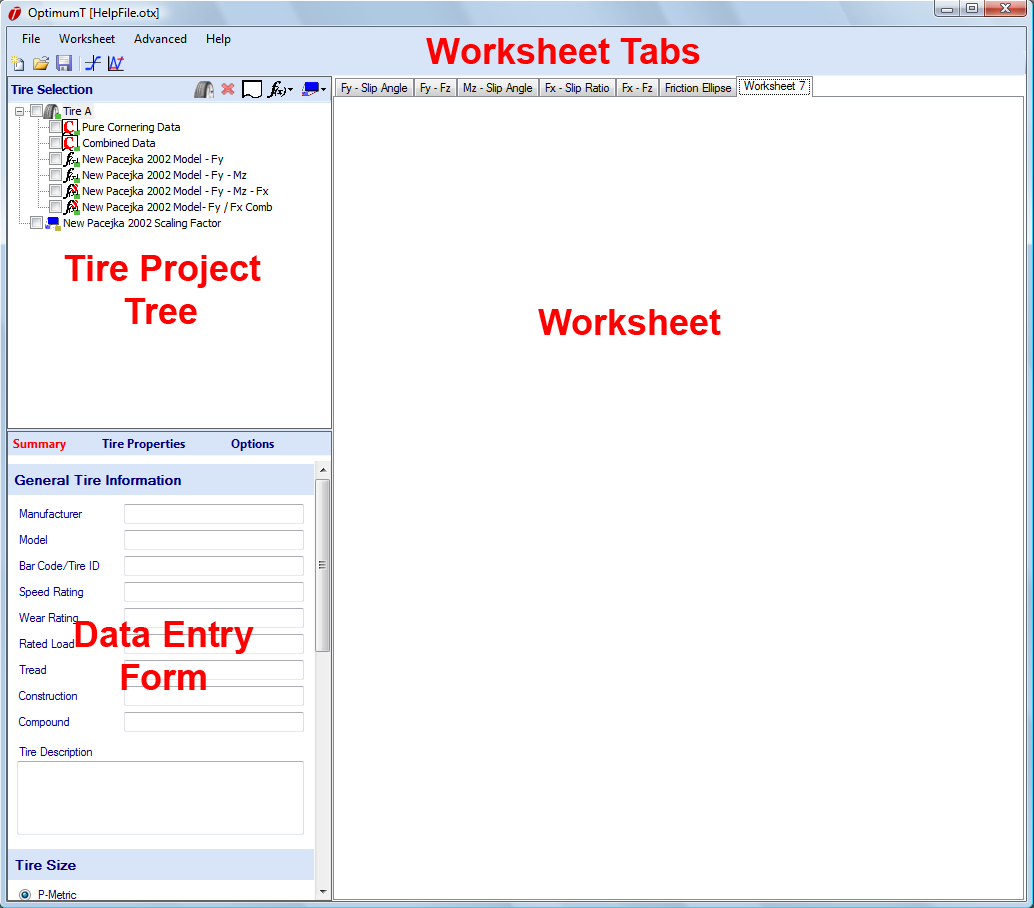
\includegraphics[width=0.95\textwidth]{ScreenLayoutLabeled.png}
	\caption{Screen Layout}
	\label{fig:ScreenLayout}
\end{figure}


\section{Tire Project Tree}
\label{sec:TireProjectTree}
The tire project tree contains all the raw data, tire models, and scaling factors contained within the OptimumTire project. Raw data and tire models are organized by the tire item. The tire items can be seen more closely in Figure~\ref{fig:ProjectTree}.

\begin{figure}[H]
	\centering
		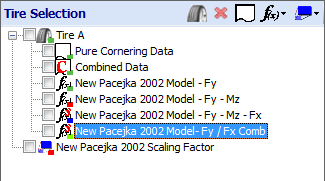
\includegraphics[width=0.95\textwidth]{ProjectTree.png}
	\caption{Project Tree}
	\label{fig:ProjectTree}
\end{figure}

The item type in the project tree can be identified by the icon to the left of the item. In Figure~\ref{fig:ProjectTree}, the first item in the list is a tire. The tire item is like a folder that contains other items in the project. Both raw data and tire models must be associated with a tire item, so this must be the first item added to a new project. This allows data and models from the same tire or construction to be grouped together.

\subsection*{Raw Data}

In Figure~\ref{fig:ProjectTree}, the first two items in the project tree under Tire A are raw data. The icon for the second item, Combined Data, has a large red "C" in it to indicate that the collapsed data is being used. Data collapsing will be explained in section~\ref{sec:DataCollapsing}. 

\subsection*{Tire Models}

The third and fourth items in this project tree are tire models. The next two items are also tire models but the red "S" in the upper right corner of the icon indicates that a scaling factor has been applied to them. 

\subsection*{Scaling Factors}

The final item is a Pacejka scaling factor. These allow the model to be adjusted without making any changes to the model coefficients. Scaling factors are discussed in more detail in section~\ref{sec:ModelScalingFactors}.
 
Like the tire item when any of the raw data, tire models, or scaling factors is clicked additional information and functionality related to the selected item will appear in the data entry form. The small color squares in the lower right corner of the icons indicate the color in which the data or model will be displayed when it is graphed. To graph a specific tire model or raw data set, check the box next to the item in the project tree (graphing is covered in section~\ref{sec:Graphing}).By right clicking on an item you can rename, delete, or copy it as well as perform other operations on it that will be discussed in later sections. 

To add items to the project, the buttons above the project tree can be used. Figure~\ref{fig:ProjectTreeButtons} shows these buttons. The three buttons furthest to the right will only be enabled when an item in the project tree is selected.

\begin{figure}[H]
	\centering
		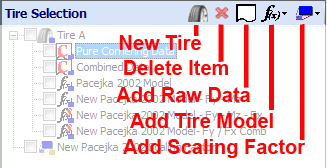
\includegraphics{ProjectTreeButtons.png}
	\caption{Project Tree Buttons}
	\label{fig:ProjectTreeButtons}
\end{figure}

\section{Data Entry Form}
\label{sec:DataEntryForm}
When an item in the project tree is clicked on, a data entry form corresponding to the project item will appear in the data entry area. Note that the name of the project item or its icon must be clicked on. Clicking on the checkbox next to the item in the project tree will not bring up the data entry form, but will change whether or not the item is to be graphed. 

Figure~\ref{fig:TireDataForm} shows an example of the data entry form. This information appears when a tire item is selected in the project tree. Information about the tire size, manufacturing, and testing procedure can be stored here.

If the raw data, tire model, or scaling factor items are selected the information in the data entry area will change to reflect these items. The tire model coefficients are also contained in this form. If a graph is clicked on, the graph setup form for that specific graph will appear in the data entry area. The data entry forms will be discussed in more detail in the chapters corresponding to these specific items.

\begin{figure}[H]
	\centering
		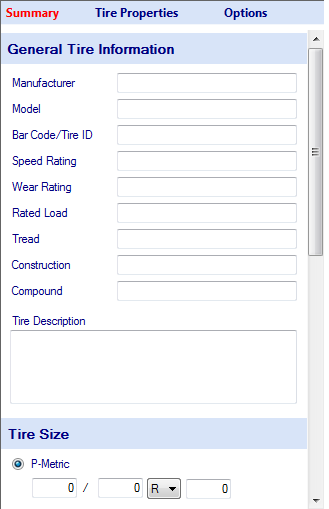
\includegraphics[width=.55\textwidth]{TireDataForm.png}
	\caption{Tire Item Data Entry Form}
	\label{fig:TireDataForm}
\end{figure}

\section{Worksheets}
\label{sec:Worksheets}
The worksheet is the area where graphs can be added to the project. Creating graphs will be covered in section~\ref{sec:Graphing}. An unlimited number of worksheets can be included in a project. To add a new worksheet, click on the \textsl{Worksheet} menu and select \textsl{New Worksheet}. Alternatively, worksheets can be added by right-clicking on the worksheet or the worksheet tabs and selecting \textsl{New Worksheet}.

Worksheets can be renamed by right-clicking on the worksheet and choosing \textsl{Rename Worksheet}. A worksheet can be deleted (and all the graphs on that worksheet) by choosing \textsl{Delete Worksheet} from the menu that appears when you right-click on a worksheet. Note that you cannot undo a delete operation.

\chapter{Raw Tire Data}
\setcounter{figure}{0}
\setcounter{table}{0}

\label{sec:RawTireData}
The raw data item in the project tree contains the imported data and provides some tools for manipulating the data. These tools allow the data to be quickly and conveniently viewed and fitted to tire models.

The raw data form, shown in Figure~\ref{fig:RawTireDataForm}, is displayed when a raw data item in the project tree is clicked on. This form has a place to store comments about the test data contained in the item. It also contains the \textsl{Data Cropping} and \textsl{Data Collapsing} tools. The \textsl{Data Cropping} tool allows user to easily view and eradicate erroneous or undesired data from the raw data. The \textsl{Data Collapsing} tool removes hysteresis from the data and separates the data into sets depending on the conditions that the tire was tested at. Once the data has been collapsed a summary of the separated data sets will appear in the table in the raw data from. The \textsl{Model Fitting} tool in this section allows you to fit the raw or collapsed data to a tire model. Tire model fitting will be covered in more detail in section~\ref{sec:TireModels}.

The Options button at the top of the raw data form allows you to add another data file, export the tire data, or access the \textsl{Data Cropping} tool. A more detailed description of these operations is included in this section. The Data Comments allow the user to enter notes and information about the data. This information will be saved with the raw data in OptimumTire.

\begin{figure}[H]
	\centering
		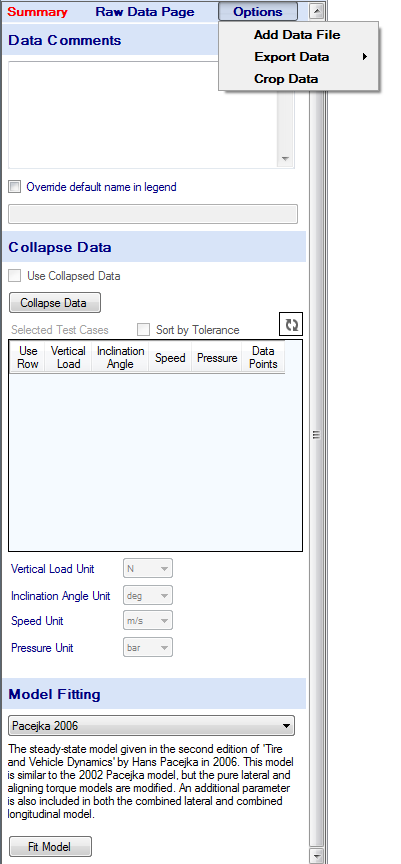
\includegraphics[height=0.95\textheight]{RawTireDataForm.png}
		\caption{Raw Tire Data Form Before Collapsing}
	\label{fig:RawTireDataForm}
\end{figure}

\section{Importing Data}
\label{sec:ImportingData}
When the \textsl{Add Raw Data} button above the project tree is clicked on, an open file window will appear. OptimumTire can open either a .rtd file, which is the OptimumTire binary format for tire data, or a CSV or ASCII file with .csv or .dat file extensions. Files with no extension are assumed to be CSV/ASCII files.

If a .rtd file is opened, the data will be automatically imported in the correct format and coordinate system. No further actions are required by the user.

If a CSV or ASCII file is selected a dialog box as shown in Figure~\ref{fig:ImportOptions} will open. In this box the the file properties can be specified. The character that separates the columns in the file and then the character that represents the decimal point should be selected. Multiple column separators can be selected if different file formats are to be used.

\begin{figure}[H]
	\centering
		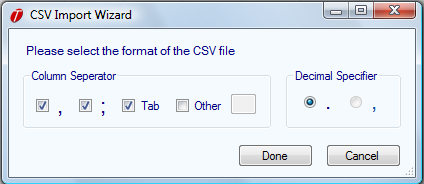
\includegraphics{ImportOptions.png}
	\caption{CSV Import Options}
	\label{fig:ImportOptions}
\end{figure}

If a CSV or ASCII file is opened, the data import wizard, shown in Figure~\ref{fig:DataImportWizard}, will appear. In this window the user specifies what quantity each column of raw data contains (i.e. SA, SR, Fx, etc) and the unit for that quantity. At the bottom of the dialog box, default values for quantities that are missing from the data can be specified. For example, if inflation pressure was not recorded in the test, the user could manually enter a constant inflation pressure to be included in the data. The coordinate system that the data was collected also needs to be specified.

\begin{figure}[H]
	\centering
		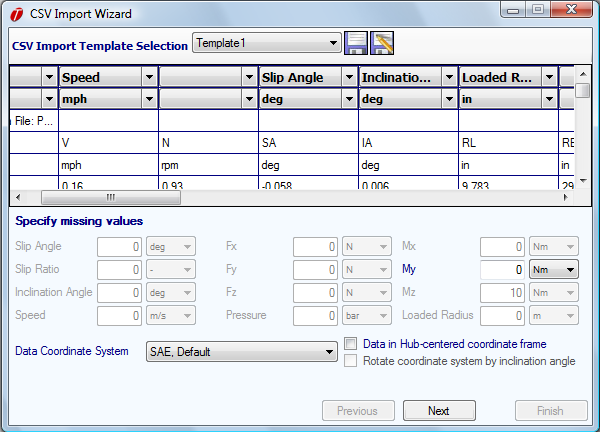
\includegraphics[width=1.0\textwidth]{DataImportWizard.png}
	\caption{Data Import Wizard}
	\label{fig:DataImportWizard}
\end{figure}

This process can be automated by using the import template feature at the top of Figure 2.1. The template to be used is chosen through the \textsl{CSV Import Template Selection} dropdown box. It can be seen in the figure that currently Template 1 is selected. New import templates can easily be created and saved. First the data quantities, units, and coordinate system are specified.  Then to save this as an import template, click the \textsl{Save as New Template} button. Import templates can also be modified and saved by using the \textsl{Save Template} button.

Typically tire data provides the force and moments at the center of the tire contact patch. However sometimes, especially with wheel force transducer data, it will be the force and moments at the wheel center. Therefore the \textit{Data in Hub-centered coordinate frame} checkbox should be selected. Then OptimumTire will transform the force and moment data to the center of the  contact patch. If this is the case the \textit{Rotate coordinate system by inclination angle} can also be selected. This should be done if the coordinate system that the force and moments were measured in are fixed to the wheel. In this case the vertical force would be in the same direction as the inclination angle and not perpendicular to the ground. Therefore if this option is selected OptimumTire will transform the forces and moments to a ground fixed coordinate system.

Once all of the column definitions have been assigned pressing the Next button will show a preview of the data to be imported. If the data to be imported is correct, clicking on Finish will import the data into OptimumTire.

Generally different sets of raw data should be imported into OptimumTire as separate files. However multiple test files can be imported and combined in OptimumTire. This can be achieved in two ways. If the files are in exactly the same format, simply select both files at the same time (use the shift or ctrl keys to choose more than one file). The import wizard will appear for the first file and the other files will be imported with exactly the same settings.

If the files are in different formate, multiple import into the same data item is done by importing the first data set as would normally be done. After this is completed, click on the data set in the project tree. Then select Add Data in the Options button in the upper right corner of the raw data form (see Figure \ref{fig:AddData}).  This will open the same CSV Import Wizard that was used previously. Follow the same steps as before and the data will be added to the previously imported set.

\begin{figure}
	\centering
		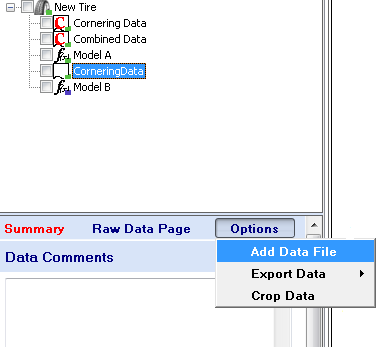
\includegraphics[width=0.50\textwidth]{AddData.png}
	\caption{Adding more data to a data set that has already been imported}
	\label{fig:AddData}
\end{figure}

\section{Importing TYDEX Data}
\label{sec:ImportingTYDEX Data}
Tire data stored in the TYDEX file format can be imported into OptimumTire. The process will load any TYDEX files the user specifies and will convert these into the CSV/ASCII format which is the default OptimumTire tire data format.

Click the \textsl{TYDEX} button in the \textsl{Add Raw Data} drop down menu to launch the TYDEX import wizard. In the window click \textsl{Add Files} to add in all the TYDEX files which should be imported. The TYDEX import will combine all the TYDEX files into a single OptimumTire tire data object which can be used for model fitting. Generally, select all TYDEX files from a single test run (multiple sweeps) in the add file dialog.

Once the files have been added they can be selected or un-selected using the checkboxes in the file list window. Un-selected files will not be included in the import process. By clicking on one of the files in the list, additional information from the TYDEX file is the displayed in the textbox. 

\begin{figure}[H]
	\centering
		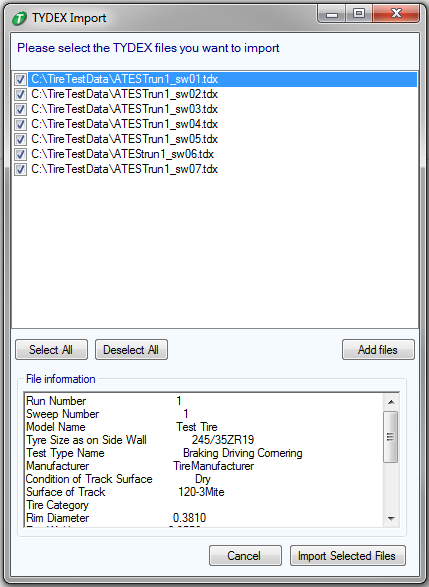
\includegraphics[width=0.5\textwidth]{TYDEXImport.png}
	\caption{TYDEX File Import Wizard}
	\label{fig:TYDEXImport}
\end{figure}

Clicking \textsl{Import Selected Files} converts the TYDEX files into a single CSV/ASCII files and the \textsl{Add Raw Data} import tool is automatically launched.

\section{Data Cropping}
\label{sec:DataCropping}
Data cropping allows the user to remove any unwanted or unnecessary data. Often in tire tests the data from conditioning or warm up procedures is included in the data file. This data can be easily removed in OptimumTire. 
The raw data can be cropped by selecting \textsl{Crop Data} under the \textsl{Options} button on the top of the raw data form. This will open the \textsl{Crop Data} window as shown in Figure~\ref{fig:DataCroppingTool}. The raw data to be cropped is displayed in the graph. You can select what properties of the raw data are graphed by selecting the checkboxes on the left. In the figure slip angle is represented by the blue line and the inclination angle by the red line. By clicking on the boxes to the right of the properties the color of the property can be changed. The values to the right of this correspond to the data values at the location of the black line on the graph. At the bottom the units of the data and the axis ranges can be changed. 

\begin{figure}[H]
	\centering
		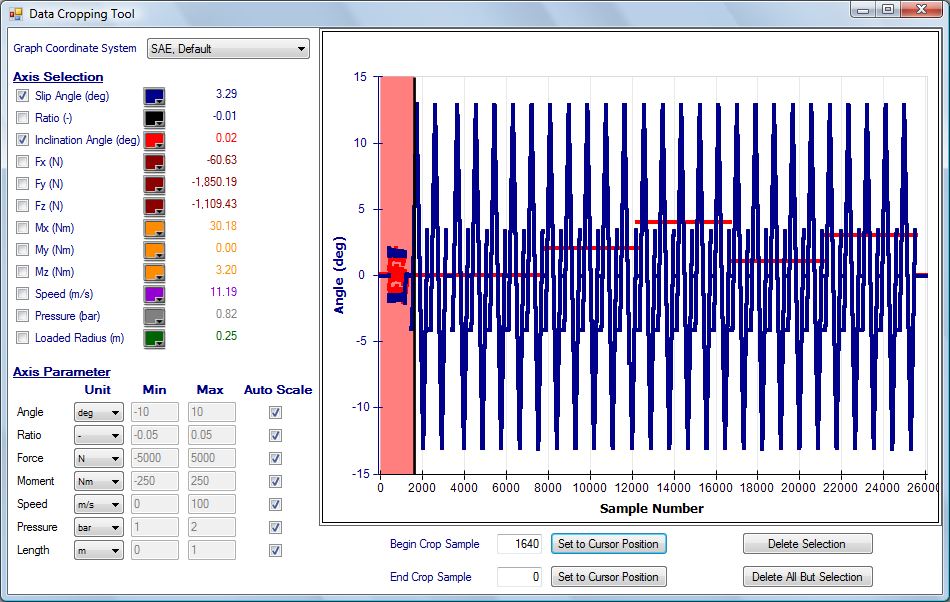
\includegraphics[width=1.0\textwidth]{DataCroppingTool.png}
	\caption{Data Cropping Tool}
	\label{fig:DataCroppingTool}
\end{figure}

As can be seen at the beginning and end of the run extra data exists that is not necessary. The data to be removed can be selected by entering the beginning and ending sample numbers in the \textsl{Begin Crop Sample} and \textsl{End Crop Sample} textboxes at the bottom of the window. Alternatively the vertical black line on the graph can be dragged to the point where the data should be cropped. Pressing the corresponding \textsl{Set} button defines the beginning or ending sample number. The background of the selected data will be pink. Then the \textsl{Delete Selection} or \textsl{Delete All But Selection} buttons can be clicked to remove the selected data. Figure \ref{fig:CroppedData} displays the data from Figure~\ref{fig:DataCroppingTool} after it has been cropped. As can be seen only the relevant test data remains. When the Crop Data is closed the program will return to the primary OptimumTire screen with cropped data.
 
 \begin{figure}[H]
	\centering
		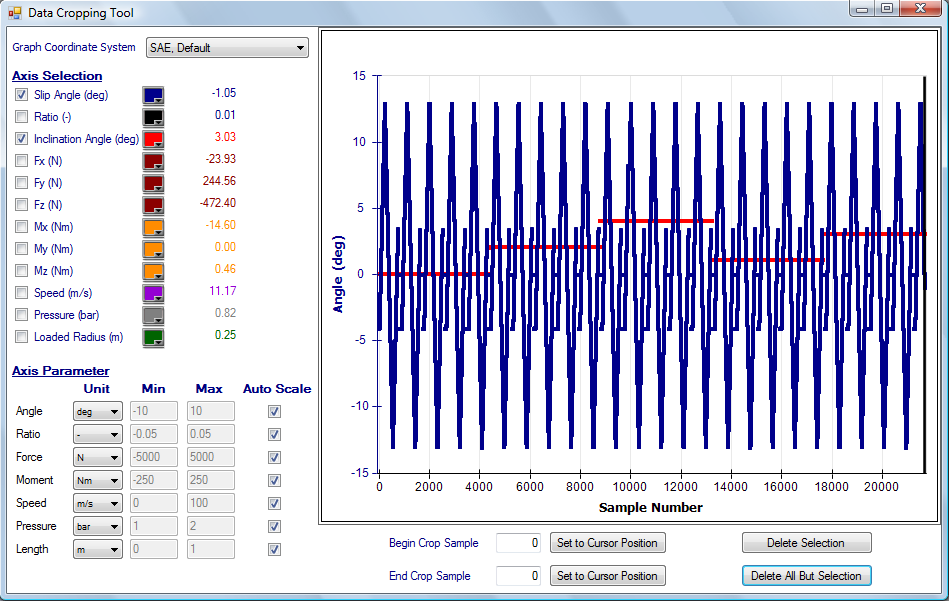
\includegraphics[width=1.0\textwidth]{CroppedData.png}
	\caption{Cropped Data}
	\label{fig:CroppedData}
\end{figure} 


\subsection{Data Cropping Templates}
\label{sec:DataCropping:templates}

To simplify the task of repetitively cropping data, templates can be set up. Crop templates record the beginning and ending sample number of each section deleted. The same actions can be applied to another data file. The file on which a template is used must be at least on long as the largest ending sample number in the template. A warning will be displayed if the crop template was created for a data file with a different number of samples than the one its being applied to. 

To record a crop template, simply crop a data file as usual. Once this is done, click on the "Save As" button next to Crop Template. Enter a name for the template and click on Save.

To use a crop template, open the Data Cropping Tool (see Section \ref{sec:DataCropping}) and choose the desired crop template from the Crop Templates List.


\section{Data Collapsing}
\label{sec:DataCollapsing}
The raw data is collapsed to remove hysteresis and variance from the test and make it easier to identify the tire test conditions. Collapsing the data allows tire models to be fit much more quickly. The following figures demonstrate this tool.Figure~\ref{fig:UncollapsedData} shows an example of raw data before it is collapsed and Figure~\ref{fig:CollapsedData} shows the same data collapsed. The data collapsing tool does not delete any data thus the original raw data is still available in OptimumTire. Therefore if desired all of the data can still be graphed or just the collapsed data.

 \begin{figure}[H]
	\centering
		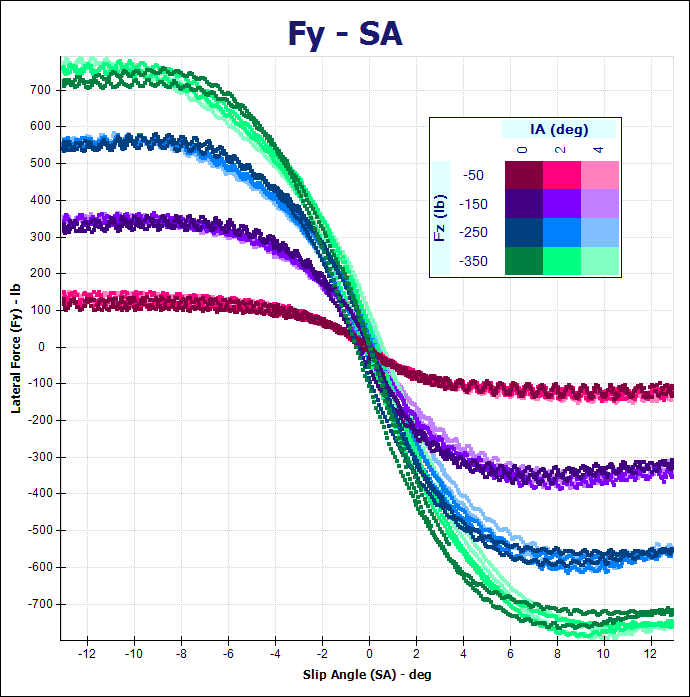
\includegraphics[width=0.9\textwidth]{UncollapsedData.png}
	\caption{Raw Data Before Collapsing}
	\label{fig:UncollapsedData}
\end{figure} 

 \begin{figure}[H]
	\centering
		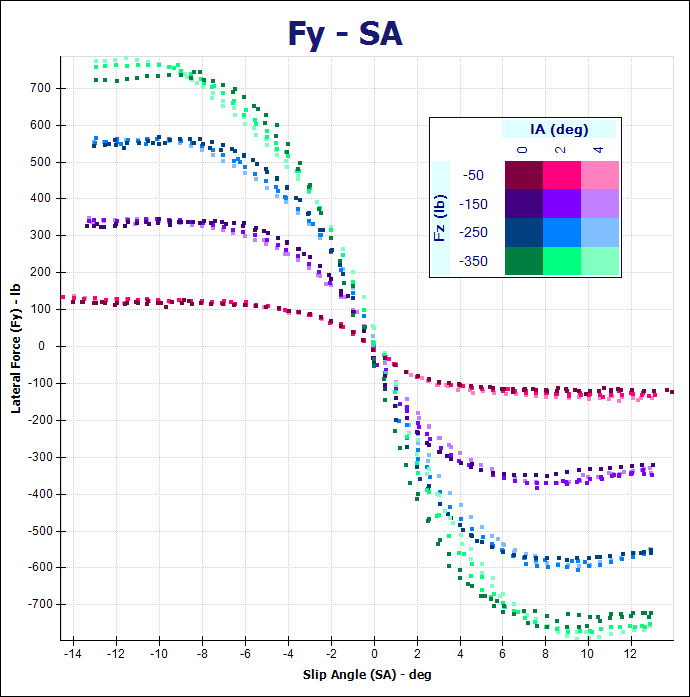
\includegraphics[width=0.9\textwidth]{CollapsedData.png}
	\caption{Collapsed Data}
	\label{fig:CollapsedData}
\end{figure} 

Now the procedure for collapsing raw data will be described. First select the raw data to be collapsed from the project tree. Then in the data entry area click on the \textsl{Collapse Data} button. This will open the data collapsing tool shown in Figure~\ref{fig:DataCollapsingTool}. 

 \begin{figure}[H]
	\centering
		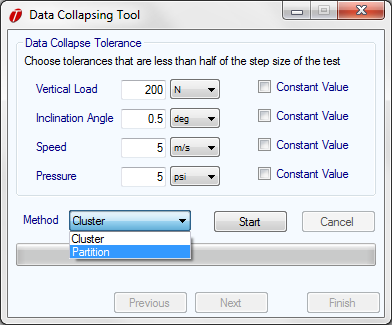
\includegraphics{DataCollapsingTool.png}
	\caption{Data Collapsing Tool}
	\label{fig:DataCollapsingTool}
\end{figure}
 
First the data is sorted into different sets depending on the test conditions. In order to do this the data collapsing tolerances should be set at less than half of the step sizes used in the tire testing. For example if a tire was tested at vertical loads of 100, 200, and 300 lbs the data tolerance should be set to at least less than 50 lbs. This will separate the different test conditions as well as sort out any irregular data. Select the constant value check box for test conditions that are kept constant throughout the test. This will increase the speed of the sorting. 

There are two sorting methods available \textsl{cluster} and \textsl{partition}. The cluster method works by creating a number of evenly spaced clusters and assigns each data point to the nearest cluster. The sizes of the initial clusters is determined by the variable tolerance. The algorithm then checks all the clusters. If the range of the cluster is too large the cluster is split if it is too small the cluster is deleted. The algorithm continues this process untill all the clusters meet the size crtieria.
The partitioning method works by assigning each data point to its own cluster. The algorithm then checks the difference between adjacent clusters if the clusters are too close they are merged. The algorithm continues until the minimum distance between clusters has met the conditions defined by the variable tolerance. 

Clicking on the \textsl{Start} button will sort the data. Once this is completed click on the \textsl{Next} button.

A list of the different sets of data will then be displayed. This is shown in Figure~\ref{fig:SortedData}. The rows of data can be sorted by value by clicking on the column headers.

It should be checked that these sets represent the data that you want to work with. Also if the data at the very beginning or end of the test was not removed with the cropping tool it can be removed here. This data will normally be at significantly different speeds or vertical loads than the rest of the data. Also if the data has a relatively low number of samples it most likely was not intended to be tested at those conditions. To remove sets of data just unselect the checkboxes next to that set. Once this is completed click on \textsl{Next}.

 \begin{figure}[H]
	\centering
		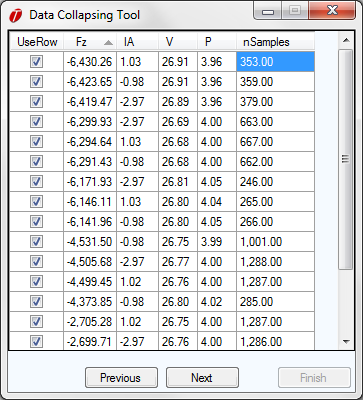
\includegraphics{SortedData.png}
	\caption{Sorted Data}
	\label{fig:SortedData}
\end{figure}

Then the discretization range over which the data will be collapsed must be selected. This is shown in Figure \ref{fig:DicretizationRange}. This determines the quantity and range of the collapsed data points that will be generated. Therefore for pure cornering data the number of steps used for the slip angle should be higher than that for the slip ratio and vice versa for the combined lateral and longitudinal data. For combined data the number of steps used should be approximately equal. 

 \begin{figure}[H]
	\centering
		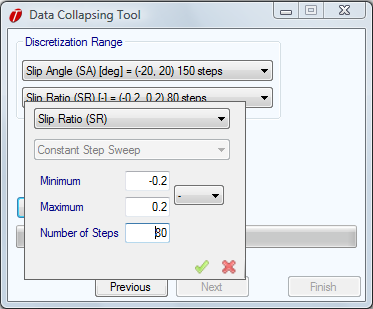
\includegraphics{DicretizationRange.png}
	\caption{Setting Discretization Range}
	\label{fig:DicretizationRange}
\end{figure}

Clicking on the \textsl{Collapse Data} button will begin the collapsing process. This will compress each set of data points that fall within each discretization step. For each step, the subsequent data points are normalized with respect to their average vertical load.   This is demonstrated in the following equations where $F_y$ is normalized with respect to the vertical load. A similar formulation is used to normalize the other output parameters (i.e.  $F_x$, $M_z$, etc�).

\begin{equation}
F_y=\frac{F_z}{F_{z0}}*F_{y0}(\alpha_0)
\end{equation}
With the normalized slip angle
\begin{equation}
\alpha_0=\frac{F_{z0}}{F_z}*\alpha
\end{equation}

Clicking on the \textsl{Finish} button will close the \textsl{Data Collapsing Tool} and return to the main OptimumTire window. A summary of the collapsed tire data will now appear in the data entry area when the tire data is selected in the project tree. The check-box labeled \textsl{Use Collapsed Data} will automatically be checked after the data is collapsed. This checkbox specifies whether the original or collapsed data will be used for graphing and fitting of tire models. This can be seen in Figure~\ref{fig:SummaryCollapsedData}.

 \begin{figure}[H]
	\centering
		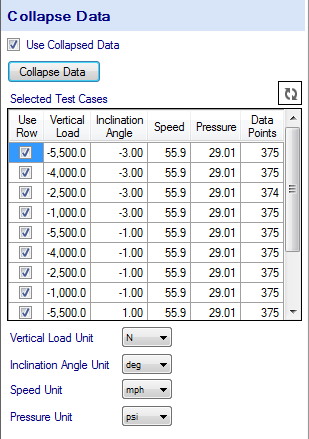
\includegraphics{SummaryCollapsedData.png}
	\caption{Summary of Collapsed Data in the Data Entry Form}
	\label{fig:SummaryCollapsedData}
\end{figure}

The summary of the collapsed data shown in Figure~\ref{fig:SummaryCollapsedData} allows the user to quickly see the data sets and the conditions of the test. The data can be sorted numerically by clicking on the column headers. The data can also be sorted by the tolerances by selecting the \textit{Sort by Tolerance} checkbox.  The checkboxes in the first column allow the user to exclude or include certain data sets from graphing and tire model fitting. Since the original raw data is still stored in OptimumTire the same data can be collapsed multiple times.

\section{Exporting Data}
\label{sec:ExportingData}
By selecting the Options-Export button at the top of the raw data entry form the tire data can be exported to an OptimumTire Raw Data File or a CSV file. After the desired format is selected a dialog box will appear. Clicking on the \textsl{Yes} button will export the cropped and collapsed tire data while clicking on the \textsl{No} button will export the raw tire data.

\chapter{Tire Models}

\label{sec:TireModels}
\setcounter{figure}{0}
\setcounter{table}{0}

Currently, nine tire models are implemented in OptimumTire:
\begin{itemize}
\item	Fiala Model
\item	Brush Model
\item Harty Model
\item	Pacejka Magic Formula '96 Model
\item	Pacejka Magic Formula 2002 Model
\item	Pacejka Magic Formula 2002 Model with Inflation Pressure effects
\item	Pacejka Magic Formula 2006 Model
\item	Magic Formula 5.2 Model
\item	Magic Formula 6.1 Model
\end{itemize}

The coefficients of these tire models can be manually inputted or imported from an OptimumTire Native File. OptimumTire can also fit these models to raw tire data. More specific information regarding the tire models is included in the section~\ref{sec:References}.

\section{Manually Input Model}
\label{sec:ManuallyInputModel}
If the tire model coefficients have already been determined, they can be manually inputted into OptimumTire. First select the \textsl{New Tire Model} button at the top of the project tree. Then choose the type of tire model you would like to add to the project. This tire model will be added to the project tree. Right clicking on the tire model allows the user to rename, delete, or copy the model as well as many other functions.
The model coefficients can now be entered into the model input form, which appears in the data entry area when the model is clicked on. An example of this form is shown in Figure~\ref{fig:TireModelForm}. For coefficients that have units the units can be specified in the dropdown boxes to the right of the value. The small plus and minus buttons also to the right of the values allow the user to adjust the model. This feature is covered in detail in section~\ref{sec:AdjustingModels}.

 \begin{figure}[H]
	\centering
		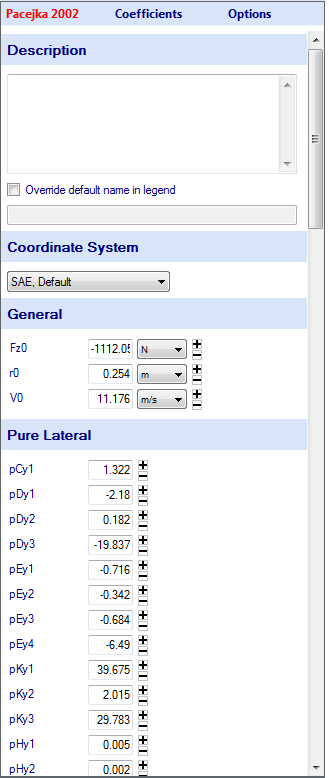
\includegraphics[height=0.95\textheight]{TireModelForm.png}
	\caption{Tire Model Input Form}
	\label{fig:TireModelForm}
\end{figure}

\section{Import and Export Models}
\label{sec:ImportandExportModels}
Before a tire model is imported into OptimumTire the appropriate tire model needs to be added to the project. This is done by clicking on the \textsl{New Tire Model} button at the top of the tire project tree. Once the tire model is added clicking on it will display its coefficients in the data entry area. Since it is a new model all of the coefficients will be zero. At the top of the data entry area click on Options-Import as shown in Figure~\ref{fig:ImportTireModel}. Tire model coefficients can then be imported from an OptimumTire Native file or from a TIR, or similar, file. Note that when you import a model, OptimumTire will overwrite the data contained in the model input form.
 


 \begin{figure}[H]
	\centering
		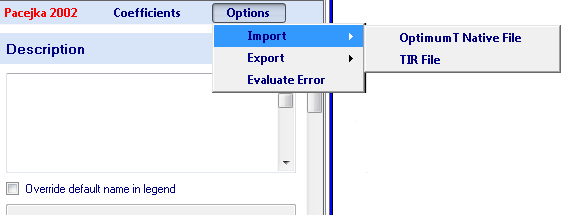
\includegraphics[width=1.0\textwidth]{ImportTireModel.png}
	\caption{Import Tire Model}
	\label{fig:ImportTireModel}
\end{figure}

Tire models can also be exported from OptimumTire by clicking on the desired tire model in the project tree. Then, at the top of the data entry area, click on \textsl{Options-Export} and select the file format you prefer. You can export to OptimumTire Native files, Excel, Lookup tables and into text-based files, such as TIR files. You also have the option of copying the tire model to the clip board for use with the addin (it will be in an encoded text format).

\begin{figure}[H]
	\centering
		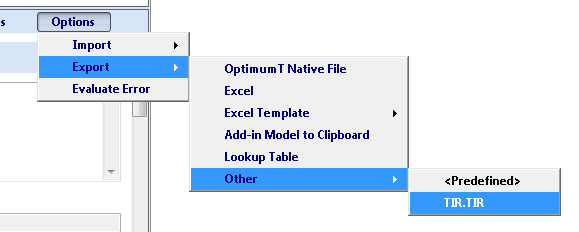
\includegraphics[width=1.0\textwidth]{ExportModel.png}
	\caption{Export Tire Model}
	\label{fig:ExportModel}
\end{figure}


\subsection{Export Templates}
\label{sec:ImportandExportModelsExportTemplate}
When exporting to a text-based format format, like a TIR file, OptimumTire uses export templates. You can edit the export templates in the template manager. When creating a new template, it is recommended that you start with an existing template and modify it. (If you start from a Predefined template, you will need to clone it first because these are read-only). When OptimumTire reads a template, it looks for parameter fields in the format \texttt{\#PARAM\#DEFAULT-VALUE\#}. Note that there are a total of three \texttt{\#} symbols for each parameter. \texttt{PARAM} denotes the name of the parameter, \texttt{DEFAULT-VALUE} denotes the default value for this parameter if it is not found in the tire model. If there are parameters specified in the export template that are not in the tire model, the user will be asked to specify them in a dialog when exporting a model. The default value will be used if the user does not specify a different value when exporting. The model description and coordinate system can be exported using the tags \texttt{\#DESC\#} and \texttt{\#COORDSYS\#} respectively.

When exporting models using templates be aware that the simulation program you intend to use the model with may require the model in a specific coordinate system. Tir and similar files do not contain coordinate system information so the coordinate system must be modified within OptimumTire before exporting. In the case of the MF5.2 and P96 templates, which have been designed for use in RaceSim, you can not export using the SAE coordinate system. It is recommended that you export using the Iso coordinate system for these models.

OptimumTire also offers the ability to export lookup tables for simulation programs that do not directly import model coefficients or equations. For more details on how to use this feature of OptimumTire see section~\ref{sec:LookupTableExport}.

\subsection{Excel Export Templates}
\label{sec:ExcelExportTemplate}
OptimumTire can also export to Microsoft Excel using export templates similar to those explained in the previous section ~\ref{sec:ModelFittingOrder}. An Excel template is a regular Excel worksheet with cells that contain text that can be recognised by OptimumTire. When OptimumTire reads an Excel template it looks for parameter fields in the format \texttt{\#PARAM\#} where PARAM is the name of the coefficient to be exported, eg. pCy1 as shown in Figure ~\ref{fig:ExcelTemplate}. The model description and coordinate system can be exported using the tags \texttt{\#DESC\#} and \texttt{\#COORDSYS\#} respectively (Note OptimumTire will only search the first worksheet of an Excel template for the parameter fields). Once the template has been created the file should be copied and pasted into the application data folder using the template manager or saved in the application data folder:

Windows Vista and Windows 7:\\
\texttt{C:\textbackslash Users\textbackslash UserName\textbackslash AppData\textbackslash Roaming\textbackslash OptimumT\textbackslash ExcelTemplates}

Windows XP:\\
\texttt{C:\textbackslash Documents and Settings\textbackslash UserName\textbackslash Application Data\textbackslash Roaming\textbackslash OptimumT\textbackslash ExcelTemplates}


\begin{figure}[H]
	\centering
		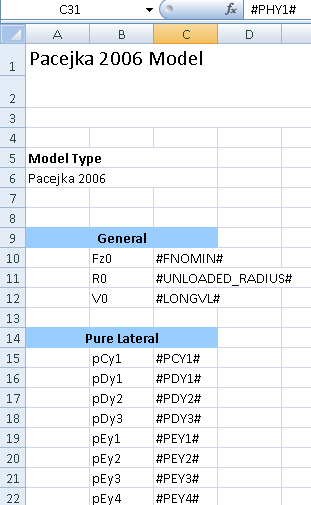
\includegraphics[width=0.5\textwidth]{ExcelTemplate.png}
	\caption{Example Excel Export Template}
	\label{fig:ExcelTemplate}
\end{figure}

\section{Fitting Models to Raw Data}
\label{sec:FittingModelstoRawData}
Before fitting a tire model to the raw data the data should be properly cropped and collapsed. This will make the fitting more accurate and significantly quicker. Also make sure that the \textsl{Use Collapsed Data} option is selected for the tire data that will be used. This can be found at the top of the \textsl{Collapse Data} section in the tire data input area.
The following sections demonstrate how to fit a tire model. This example will use pure lateral and combined longitudinal and lateral data to create a complete tire model. Depending on the data available and the goal of the model fitting the order in which the models are fit can vary. More information about the order the models should be fit is included in section~\ref{sec:ModelFittingOrder}.

\subsection{Pure Lateral Model}
\label{sec:PureLateralModel}
Fitting of the cornering data to the model lateral force coefficients is generally done first. To begin select the tire data to be modeled in the project tree. Go to the last section of the data entry area, labeled \textsl{Model Fitting}. This is shown in Figure~\ref{fig:TireModelSelection}. In the drop down box select the type of tire model to be fitted. Once you have selected the type of model to be used click the \textsl{Fit Model} button. This will open the Model Fitting Tool as can be seen in Figure~\ref{fig:ModelFittingSelection}. 

 \begin{figure}[H]
	\centering
		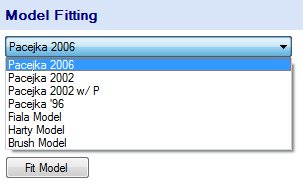
\includegraphics{TireModelSelection.png}
	\caption{Selecting the Tire Model to be Fit}
	\label{fig:TireModelSelection}
\end{figure}

\subsection*{Specify Coefficients to be Calculated}
In the \textsl{Model Fitting Selection} window the coefficients to be fit are selected. The coefficients that the error calculation is based on are also selected by choosing the \textsl{Fit and Calculate Error} option in the dropdown boxes.  For this case you would select \textsl{Fit and Calculate Error} in the drop down box labeled Fy Pure as is shown in Figure~\ref{fig:ModelFittingSelection}. \textsl{Fit and Calculate Error} must always be selected for at least one of the sets of coefficients. At the bottom of this window the coordinate system of the model can be selected.  To proceed click the Next button.

 \begin{figure}[H]
	\centering
		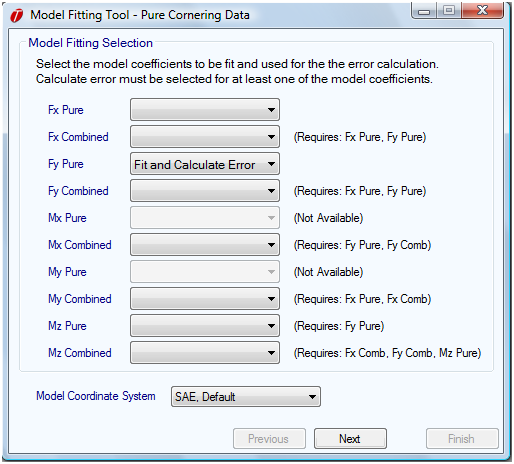
\includegraphics{ModelFittingSelection.png}
	\caption{Model Fitting Selection}
	\label{fig:ModelFittingSelection}
\end{figure}

\subsection*{Model Constraints}
Now the model constraints must be set. The constraints required vary depending on what type of model is being fit. For the Pacejka models the constraints include the nominal (rated) tire load, $F_{z0}$, the unloaded tire radius, $R_0$, the reference velocity, $V_0$, and the reference pressure, $P_0$. Typically the nominal load is set to the largest or second largest load that the tire was tested at, the reference velocity is set to the test velocity, and the reference pressure is set to the highest inflation pressure the tire was tested at. More information regarding these parameters is included in section~\ref{sec:References}.

 \begin{figure}[H]
	\centering
		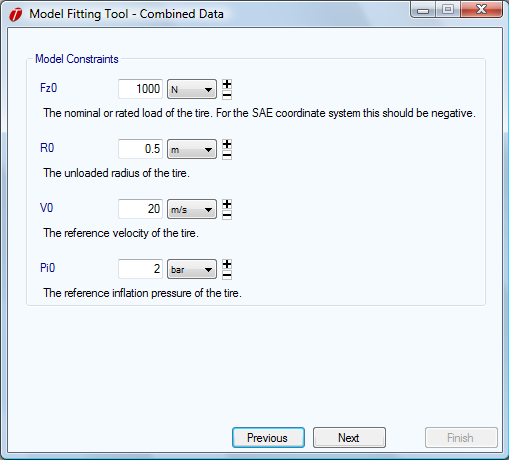
\includegraphics[width=1.0\textwidth]{Constraints.png}
	\caption{Model Constraints}
	\label{fig:Constraints}
\end{figure}

\subsection*{Define the Coefficient Boundary}
Now the \textsl{Coefficient Boundary} to be used in the fitting must be set. The coefficient boundary allows the solver to begin fitting the model in a restricted, more accurate range of values for the coefficients. However, the solver is not necessarily restricted to the range of coefficients set by the boundaries.  In Figure~\ref{fig:CoefficientBoundaries} the Coefficient Boundary window is shown. A \textsl{Coefficient Boundary} is chosen by selecting it from the list. Click on \textsl{Next} to proceed.

\begin{figure}[H]
	\centering
		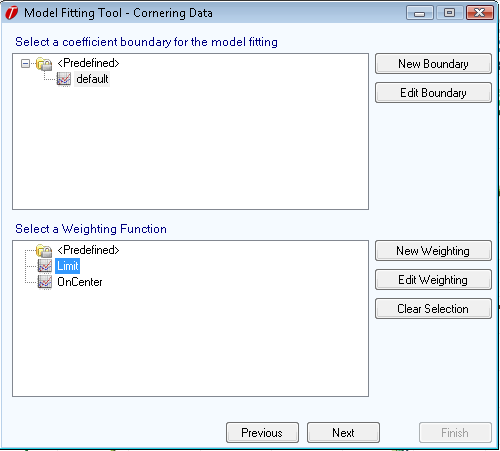
\includegraphics[width=1.0\textwidth]{CoefficientBoundaries.png}
	\caption{Coefficient Boundary}
	\label{fig:CoefficientBoundaries}
\end{figure}

Coefficient boundaries can easily be created or edited by clicking on the \textsl{New Boundary} and \textsl{Edit Boundary} buttons to the right. However the coefficients in the \textsl{Predefined Folder} cannot be modified. If they are edited, the edited version will be saved outside of the \textsl{Predefined} folder and the original version will stay unchanged.  When these buttons are clicked the \textsl{Coefficient Boundary Editor} window will open as shown in Figure~\ref{fig:NewCoefficientBoundary}. This window allows the boundaries for each coefficient to be changed. If the \textsl{Hard Boundary} check boxes are selected the solver will be restricted to finding a solution within this range of coefficients. Save the new or edited boundary by typing in a name at the top of the window and clicking on save. Now you can close this window and the new boundary will be available for selection in the \textsl{Coefficient Boundary} window.

\begin{figure}[H]
	\centering
		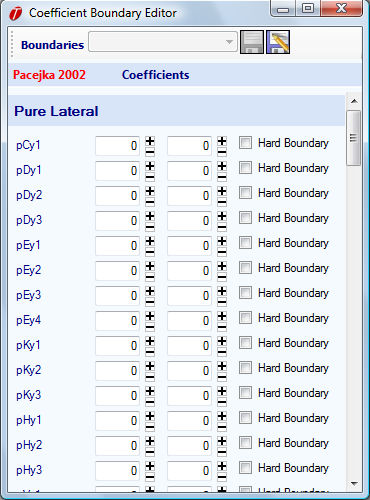
\includegraphics{NewCoefficientBoundary.png}
	\caption{Coefficient Boundary Editor}
	\label{fig:NewCoefficientBoundary}
\end{figure}


\subsection*{Weighting Functions}
Optionally, you can select a weighting function to apply to the fit. This will change the way the error is evaluated. For details about the error evaluation, please see Section \ref{sec:models:solverparameters}. You can select an existing weighting function by selecting it from the list in the coefficient boundary selection dialog (Figure \ref{fig:CoefficientBoundaries}). You can also create a new weighting function or edit an existing one in this dialog. If you have selected a weighting function and wish to remove this selection, click the \textit{Clear Selection} button.

\begin{figure}[H]
	\centering
		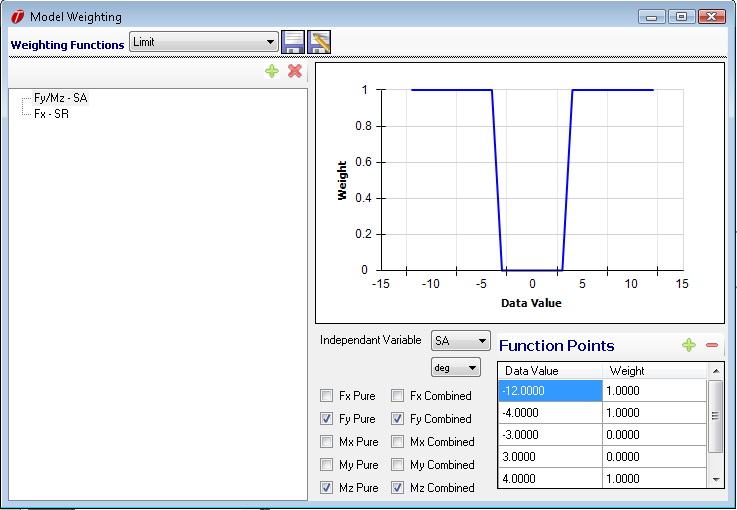
\includegraphics[width=0.90\textwidth]{WeightingFunction.png}
	\caption{The weighting function editor}
	\label{fig:WeightingFunction}
\end{figure}

Figure \ref{fig:WeightingFunction} shows the weighting function editor. It is accessible by clicking either the \textit{New Weighting} or \textit{Edit Weighting} button. At the very top of the dialog, you can save or load a weighting function. On the left side, you can select the \textit{Weighting Pages} which define a part of a weighting function. There is no limit to the number of weighting pages that you can add (though there is a practical limit of 60, as it is not possible to define more than 60 non-redundant weighting pages). Each weighting page has one independent variable one ore more dependent variables. If you want to make the solver treat the error of the FxPure fit with more "importance" at high slip ratios, you would define the independent variable to be slip ratio (SR) and the dependent variable to be FxPure. A given pair of independent and dependent variables cannot be defined twice within the same weighting function. You will receive an error if you try to do this.

Once the independent and dependent variables have been selected for a weighting page, the values of the weighting function can be entered. The function is defined as a table. OptimumTire will do a linear interpolation between the entries in the table. The \textit{Data Value} column indicates the values of the independent variable, and the \textit{Weight} column defines the weight. Typically the values in the weight column will be between $0$ and $1$.



\hypertarget{models:solverparameters}{\subsection*{Solver Parameters and Error Evaluation}}\label{sec:models:solverparameters}
Next the \textsl{Population} and \textsl{Iterations} needs to be set. These parameters are used by the solver and are not related to the tire models.  The \textsl{Population} is the number of initial vales that the solver will distribute between the coefficient boundaries. Therefore if the coefficient boundaries are well defined the population can be less and vice versa.\textsl{ Iterations} are the number of steps the solver will take when fitting the model.  With a more complex model a larger number of iterations is required. The window that these parameters are set is shown in Figure~\ref{fig:SolverParameters}.

 \begin{figure}[H]
	\centering
		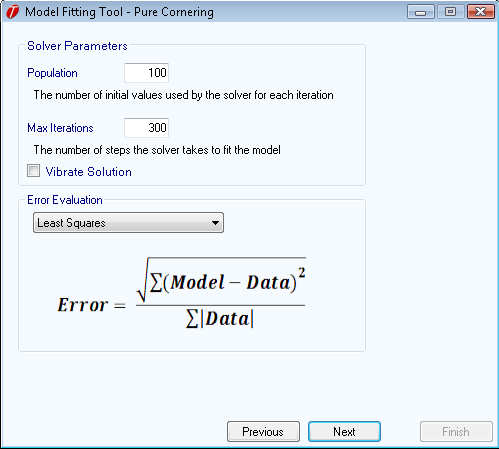
\includegraphics[width=1.0\textwidth]{SolverParameters.png}
	\caption{Solver Parameters and Error Evaluation}
	\label{fig:SolverParameters}
\end{figure}

The \textsl{Vibrate Solution} option will cause a small random variation to be applied to the data at each step. This can help the solver converge towards a global minimum slightly faster. Statistically, the variation is applied equally in both direction, so this technique does not bias the results.

The \textsl{Error Evaluation} can now be selected. This determines what type of error criteria is used when fitting the model. The four types of error criteria included in OptimumTire are described below. In the equations \textsl{Model} represents the value found by the model fitter and \textsl{Data} represents the value of the actual raw data.

\begin{itemize}
\item Least Squares Error:
\begin{displaymath}
Error=\frac{\sqrt{\sum\left(Model-Data\right)^2}}{\sum\left|Data\right|}
\end{displaymath}

\item	Normalized Least Squares Error:
\begin{displaymath}
Error=\frac{\sqrt{\sum\left(\frac{Model-Data}{Data}\right)^2}}{\# of data points}
\end{displaymath}

\item	Total Error:
\begin{displaymath}
Error=\frac{\sum\left|Model-Data\right|}{\sum\left|Data\right|}
\end{displaymath}

\item	Normalized Total Error:
\begin{displaymath}
Error= \frac{\sum\left|\frac{Model-Data}{Data}\right|}{\# of data points}
\end{displaymath}
\end{itemize}

Typically the \textsl{Least Squares Error} criteria will result in the best overall model fit. However depending on the variance and testing conditions of the raw data some of the other error criteria may produce a better fit. For example when fitting an aligning torque model \textsl{Total Error} will often produce slightly better results. The \textsl{Normalized Error} criteria gives equal weight to all of the data points. Therefore it will improve the model fitting at lower loads.

In the case that a weighting function is used, the error evaluation is modified to be the following. The weightin is denoted as $w_i$ and is evaluated for each data point separately.

\begin{itemize}
\item Least Squares Error:
\begin{displaymath}
Error=\frac{\sqrt{\sum w_i \left(Model-Data\right)^2}}{\sum\left|Data\right|}
\end{displaymath}

\item	Normalized Least Squares Error:
\begin{displaymath}
Error=\frac{\sqrt{\sum w_i \left(\frac{Model-Data}{Data}\right)^2}}{\# of data points}
\end{displaymath}

\item	Total Error:
\begin{displaymath}
Error=\frac{\sum w_i \left|Model-Data\right|}{\sum\left|Data\right|}
\end{displaymath}

\item	Normalized Total Error:
\begin{displaymath}
Error= \frac{\sum w_i \left|\frac{Model-Data}{Data}\right|}{\# of data points}
\end{displaymath}
\end{itemize}


\subsection*{Model Fitting}
Now OptimumTire is ready to fit the tire model. However, if something is incorrect or the user would like to change some of the settings the \textsl{Previous} button can be used to go back to the previous windows. Alternatively, the \textsl{Model Fitting Tool} window can be closed and the model fitting restarted.

Clicking on the \textsl{Summary} button allows the user to check to make sure all of the solver settings are correct. It will show the model being fit, the raw data to be used, the error calculation method, the coefficient boundary, and the solver parameters selected.  To return to the \textsl{Model Fitting Tool} window just close the model summary. Once the model fitting is finished this information will be automatically transferred into OptimumTire and will be stored with the associated tire model in the models data entry form.

Clicking on the \textsl{Start} button in the upper right corner of the window will start the solver. Figure~\ref{fig:ModelFitting} shows this window after a fitting has been completed. The graph shows the convergence of the solution and the textbox shows the current error as the model is fitted. When the final solution is found click on the \textsl{Finish} button to return to the main screen of OptimumTire.

 \begin{figure}[H]
	\centering
		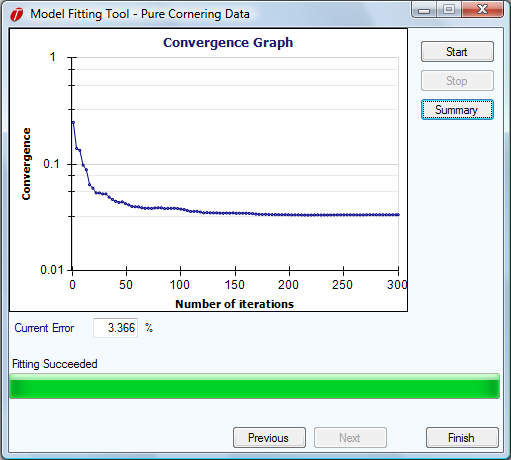
\includegraphics[width=1.0\textwidth]{ModelFitting.png}
	\caption{Model Fitting Convergence and Error}
	\label{fig:ModelFitting}
\end{figure}

The newly created tire model should now appear in the project tree. This model can now be graphed by selecting the check box next to it (Graphing is covered in Chapter~\ref{sec:AdditionalFeatures}). It should be compared to the raw data to ensure accuracy. Lateral force as a function of the slip angle at the tested inclination angles should be graphed and compared to the raw data as shown in Figure~\ref{fig:FySA}. Also the lateral force as a function of the normal load, Fz, for several slip angles should be graphed as in Figure~\ref{fig:FyFz}. The graphs should be checked for accuracy by comparing them with the raw data. The model should also be checked to ensure the curves are well behaved outside of the measurement area. This is especially important if the tire models are going to be used for simulation. Refer to section~\ref{sec:AdjustingModels} for information on adjusting the tire model.

 \begin{figure}[H]
	\centering
		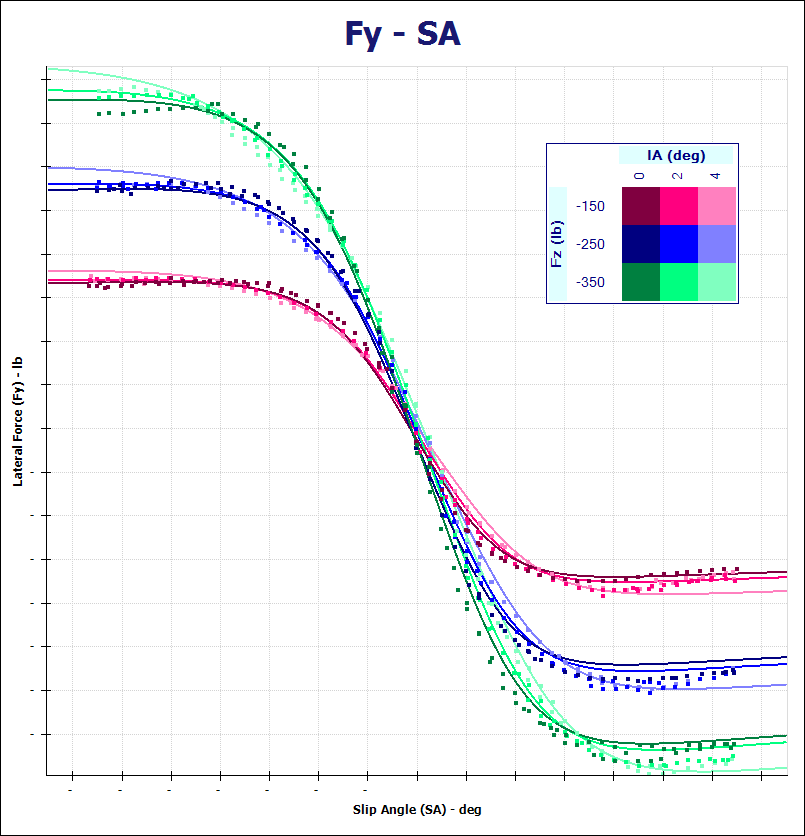
\includegraphics[width=1.0\textwidth]{FySA.png}
	\caption{Lateral Force vs. Slip Angle at Different Inclination Angles}
	\label{fig:FySA}
\end{figure}

 \begin{figure}[H]
	\centering
		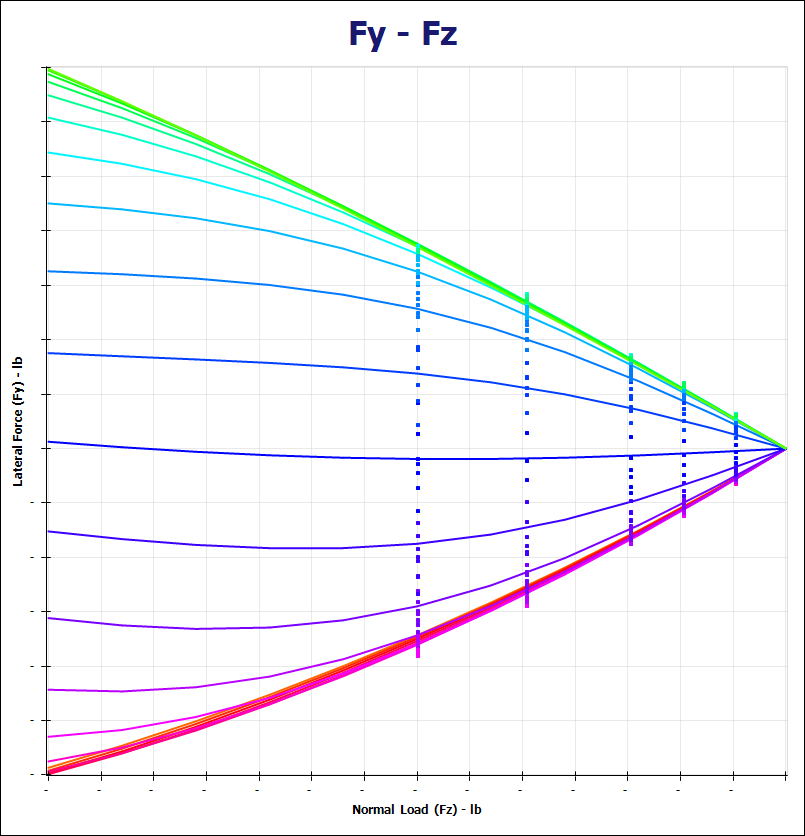
\includegraphics[width=1.0\textwidth]{FyFz.png}
	\caption{Lateral Force vs. Normal Load at Different Slip Angles}
	\label{fig:FyFz}
\end{figure}

\subsection{Aligning Torque Model}
\label{sec:AligningTorqueModel}
Fitting the aligning torque model is very similar to the lateral force model. However, there are a few small differences since this model will be combined with the lateral force model.

First select the tire data used to fit the lateral force model. In the \textsl{Model Fitting} section select the same type of tire model as was used for the lateral force model and click on the \textsl{Fit Model} button. This will open a different window than before since another tire model already exists in this project. Figure~\ref{fig:AdvancedFitting} shows the \textsl{Advanced Fitting Options} window.  In this window coefficients that were already determined in previously created models can be fixed for the current fitting. So for this example you would set the \textsl{Fy Pure} category to the previously created tire model. In later sections you will see that you can set multiple sets of coefficients and also include model scaling factors. Once the correct coefficients are selected click on the \textsl{Done} button.

 \begin{figure}[H]
	\centering
		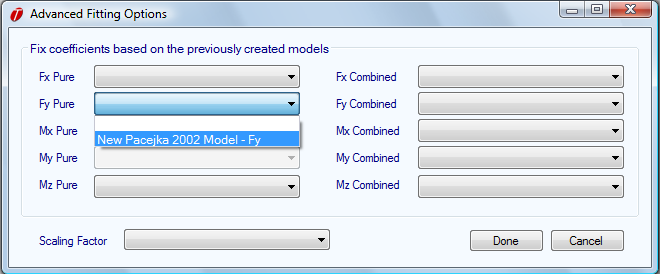
\includegraphics[width=1.0\textwidth]{AdvancedFitting.png}
	\caption{Advanced Fitting Options}
	\label{fig:AdvancedFitting}
\end{figure}

Now the \textsl{Model Fitting Selection} window that was used to fit the previous models will open. For this case \textsl{Calculate and Fit Error} in the drop down box labeled \textsl{Mz Pure} would be selected. As can be seen in Figure~\ref{fig:MzPureFit} the dropdown box corresponding to \textsl{Fy Pure} is disabled because the coefficients for this model were fixed in the previous step. The rest of the tire model can now be created in the same way as the lateral force model. When finished a new tire model will be created that contains both the pure lateral force and the aligning torque coefficients.
 
The aligning torque model could also have been created at the same time as the pure lateral force model, but for demonstration purposes was done separately. This would of have been achieved by selecting \textsl{Fit} or \textsl{Fit and Calculate Error} for both \textsl{Fy Pure} and \textsl{Mz Pure} when the coefficients to be fit were specified.
 The aligning torque as a function of the slip angle should be graphed with the tire data to check the accuracy of the model. An example of this is shown in Figure~\ref{fig:MzSA}.

 \begin{figure}[H]
	\centering
		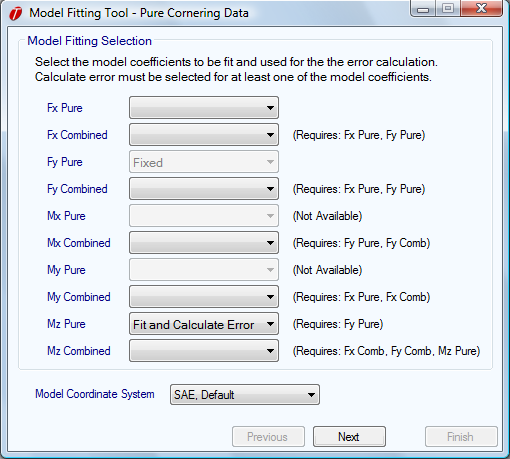
\includegraphics[width=1.0\textwidth]{MzPureFit.png}
	\caption{Specify Coefficients to be Fit}
	\label{fig:MzPureFit}
\end{figure}

 \begin{figure}[H]
	\centering
		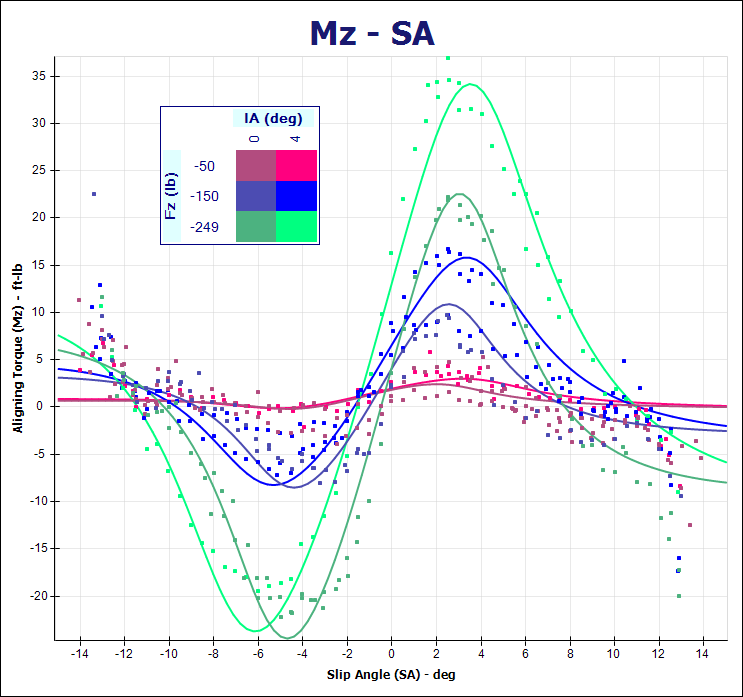
\includegraphics[width=1.0\textwidth]{MzSA.png}
	\caption{Aligning Torque vs. Slip Angle at Different Inclination Angles}
	\label{fig:MzSA}
\end{figure}

\label{sec:ModelScalingFactors}
\subsection{Model Scaling Factors}

In order to combine the data from a pure cornering test and a combined lateral and longitudinal test it will often be required to use a scaling factor.  It will adjust the pure lateral force model created from the cornering data to match the combined lateral and longitudinal data at zero slip ratio.

Figure~\ref{fig:UnscaledData} shows the discrepancy between the lateral force model and the combined data for the same tire. The pure lateral force model is represented by the solid lines and the combined data is the clusters of points at approximately 0, 3, and 6 degrees of slip angle. These points represent the force at zero slip ratio. This discrepancy is an effect of the pure cornering test being performed at a constant slip ratio and varying slip angle, while the combined test is performed at a constant slip angle with a varying slip ratio. These tests are also often performed at different speeds. Additionally, the tire will experience different heat cycling in these tests and therefore different results would be produced.

 \begin{figure}[H]
	\centering
		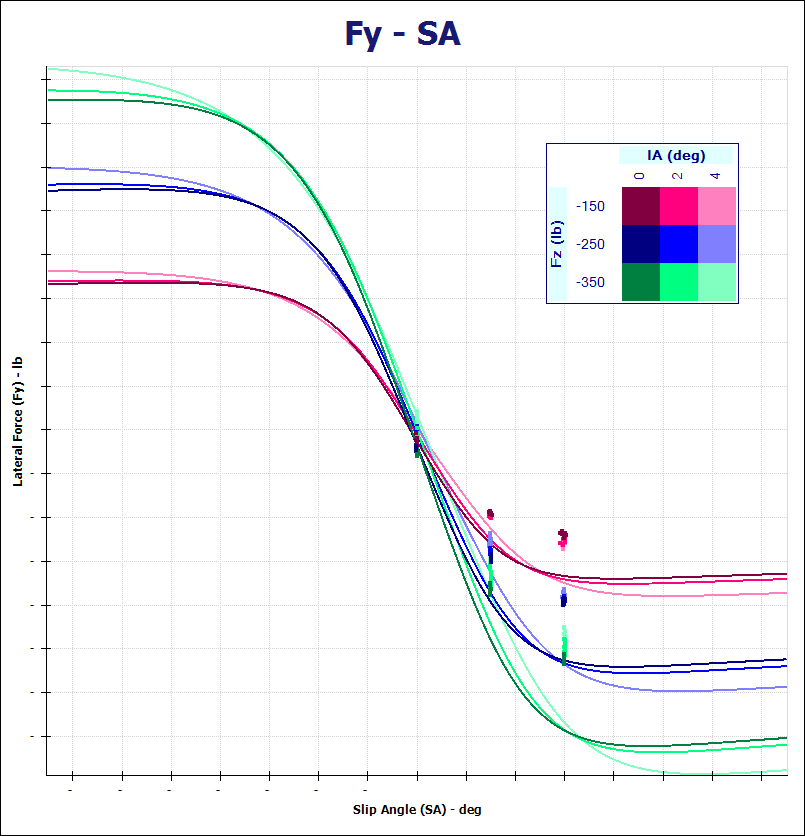
\includegraphics[width=1.0\textwidth]{UnscaledData.png}
	\caption{Lateral Force vs. Slip Angle for the Model and Data before Scaling}
	\label{fig:UnscaledData}
\end{figure}

Therefore to remedy this problem a scaling factor will be created and applied to the previously created models. To create a scaling factor click on the \textsl{New Scaling Factor} button in the upper right corner of the project tree area. Figure 3.16 shows this button, circled in red. Scaling factors can only be created for the Pacejka models. Similarly to the tire data and models, the scaling factor can be deleted, copied, or renamed by right clicking on it in the project tree.
 
In Figure~\ref{fig:NewScalingFactor} a previously added scaling factor can be seen in the project tree. The scaling factor can be applied to a tire model by dragging and dropping it onto the tire model or by right clicking on the tire model and choosing \textsl{Add Scaling Factor}. The small red "S" that appears on the selected tire model indicates that a scaling factor has been applied to the model. The scaling factor applied to a tire model can be removed or viewed by right clicking on the tire model.

 \begin{figure}[H]
	\centering
		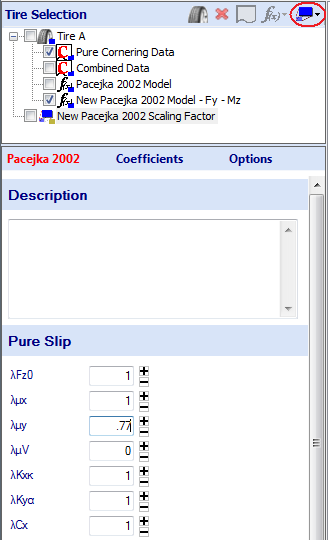
\includegraphics{NewScalingFactor.png}
	\caption{New Scaling Factor}
	\label{fig:NewScalingFactor}
\end{figure}

When a scaling factor is selected in the project tree its coefficients will appear in the data entry area as can also be seen in Figure~\ref{fig:NewScalingFactor}. A description of these coefficients appears in Table~\ref{tbl:PacejkaScalingCoefficients}. The coefficients can be modified manually or by double clicking on the "+" or "-". This will increase or decrease the value of the scaling factor by 10\%. If the scaling factor is applied to a graphed model holding down on these buttons will show a preview of the change (For more information on adjusting models refer to section~\ref{sec:AdjustingModels}). Decreasing the peak lateral friction coefficient, $\lambda\mu y$, will decrease the lateral force of the model. Figure~\ref{fig:ScaledModel} shows the lateral force of the model and data shown in Figure~\ref{fig:UnscaledData}.

 \begin{figure}[H]
	\centering
		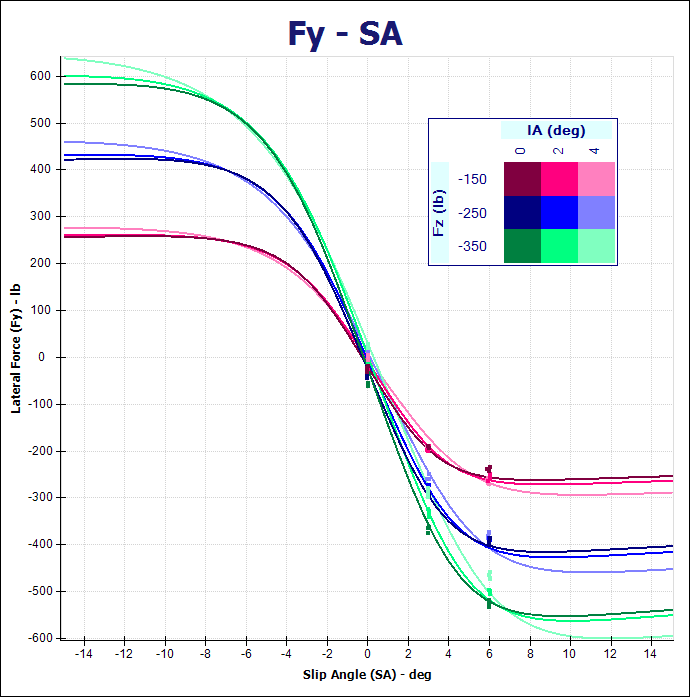
\includegraphics[width=1.0\textwidth]{ScaledModel.png}
	\caption{Lateral Force vs. Slip Angle for the Model and Data after Scaling}
	\label{fig:ScaledModel}
\end{figure}

Scaling factors are also commonly used to adjust tire models to more accurately represent the actual vehicle performance. This is necessary because the conditions and surfaces the tires are tested on are typically different than those they are to be used on. For more information regarding the scaling coefficients and their effect on the models please refer to the section~\ref{sec:PacejkaScalingFactors}.

\subsection{Pure and Combined Longitudinal Model}
\label{sec:PureandCombinedLongitudinalModel}
Now that the previously created model is properly scaled a pure longitudinal and combined longitudinal model can be created. This process will be similar to the previous models but both models will be created simultaneously. They will be created at the same time because the combined lateral and longitudinal tire data is collected at various slip angles. Thus the tire data is representative of pure and combined longitudinal force.

First, the combined data to be used should be imported and properly collapsed (These operations are covered in section~\ref{sec:RawTireData}). Then select the combined lateral and longitudinal tire data in the project tree. In the \textsl{Model Fitting} section select the appropriate tire model and click on the \textsl{Fit Model} button. This will open the \textsl{Advanced Fitting Options Window}. Set the dropdown boxes corresponding to \textsl{Fy Pure} and \textsl{Mz Pure} to the appropriate tire model to fix these coefficients. Click \textsl{Done} once this is completed.

The \textsl{Model Fitting Selection} window will now open. For this case you would select \textsl{Fit} in the \textsl{Fx Pure} drop down box and \textsl{Fit and Calculate Error} in the \textsl{Fx Combined} drop down box as shown in Figure~\ref{fig:MultipleModels}. You can also calculate the combined error for both models by selecting \textsl{Fit and Calculate Error} for both models. \textsl{Fit and Calculate Error} must be selected for at least one of the models. The rest of the tire model can now be created in the same way as the lateral force model. When finished a new tire model will be created that contains both the pure and combined longitudinal force coefficients.

 \begin{figure}[H]
	\centering
		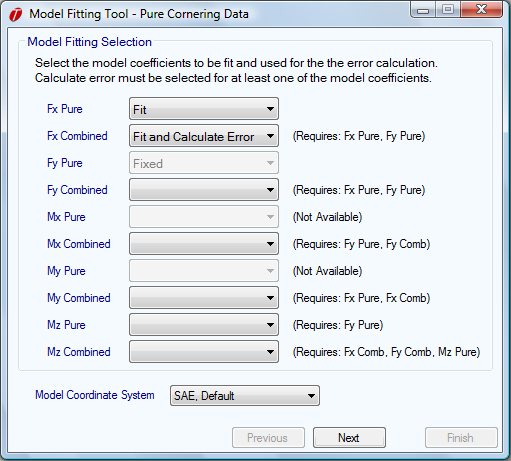
\includegraphics[width=1.0\textwidth]{MultipleModels.png}
	\caption{Fitting Multiple Models Simultaneously}
	\label{fig:MultipleModels}
\end{figure}

This model should be checked by graphing the longitudinal force as a function of the slip ratio and as a function of the normal load, Fz. Examples of these graphs are shown in Figure~\ref{fig:FxSR} and Figure~\ref{fig:FxFz}. You should check that the model curves correlate well to the tire data and are well behaved outside of the measurement area especially if the tire model is going to be used for simulation. If the models need to be adjusted please refer to section~\ref{sec:AdjustingModels}.

 \begin{figure}[H]
	\centering
		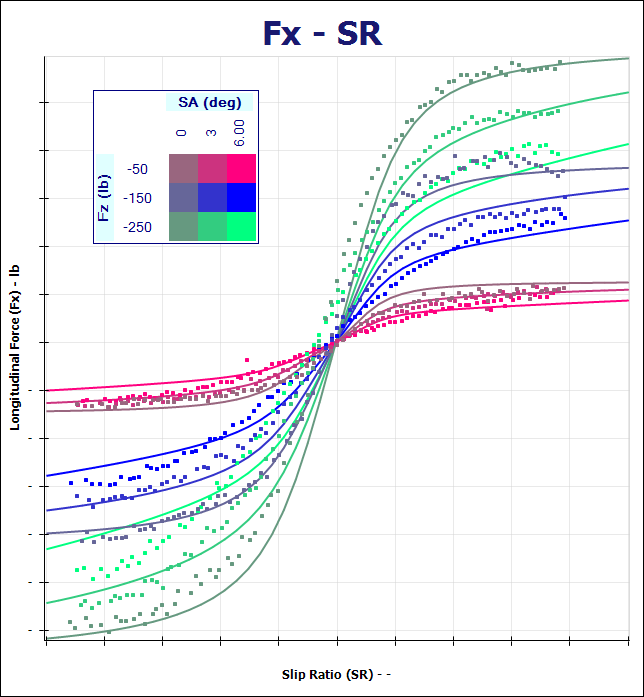
\includegraphics[width=1.0\textwidth]{FxSR.png}
	\caption{Longitudinal Force vs. Slip Angle at Different Slip Angles}
	\label{fig:FxSR}
\end{figure}

\begin{figure}[H]
	\centering
		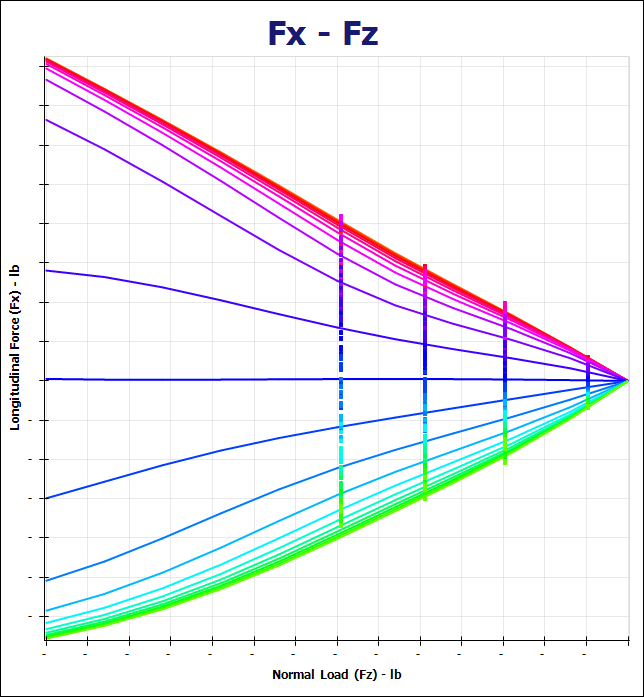
\includegraphics[width=1.0\textwidth]{FxFz.png}
	\caption{Longitudinal Force vs. Normal Load at Different Slip Ratios}
	\label{fig:FxFz}
\end{figure}

\subsection{Combined Lateral Model}
\label{sec:CombinedLateralModel}
The combined lateral model is also fit from the combined lateral and longitudinal data. The procedure is very similar to the other models except that the scaling factor should be applied when the model is fit. This is the case because the model will be based on the unscaled Fy Pure coefficients. This is done by selecting the appropriate scaling factor in the \textsl{Advanced Fitting Options} as is shown in Figure~\ref{fig:FittingwithScalingFactor}. As can also be seen in the figure all of the previously determined coefficients are set to the appropriate tire model.

\begin{figure}[H]
	\centering
		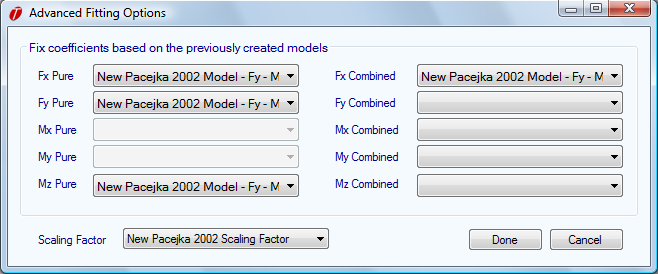
\includegraphics[width=1.0\textwidth]{FittingwithScalingFactor.png}
	\caption{Fitting with a Scaling Factor}
	\label{fig:FittingwithScalingFactor}
\end{figure}

A friction ellipse can now be plotted to ensure the accuracy of the combined lateral and longitudinal models. A graph of a friction ellipse is shown in Figure~\ref{fig:FrictionEllipse}. If these models are to be used for simulation it is very important to check that the model curves are well behaved outside of the measurement area.

\begin{figure}[H]
	\centering
		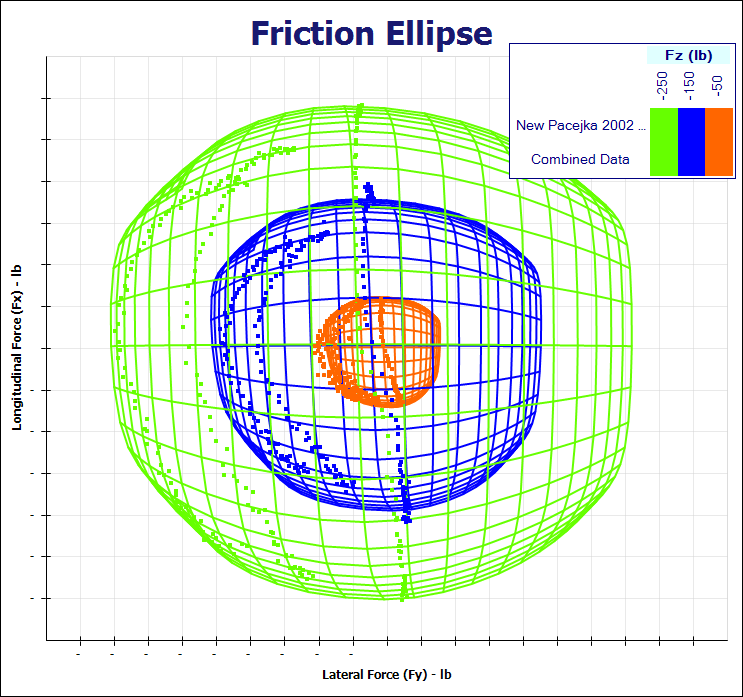
\includegraphics[width=1.0\textwidth]{FrictionEllipse.png}
	\caption{Friction Ellipse}
	\label{fig:FrictionEllipse}
\end{figure}

\subsection{Additional Models}
\label{sec:AdditionalModels}
Additional tire properties can also be fitted to the Pacejka models. These include combined models of aligning torque, rolling resistance, and overturning moment. Table~\ref{tbl:PacejkaModels} summarizes all of the models that can be fit to Pacejka coefficients in OptimumTire. It also shows what models are required before creating a new model. The required models can either be fixed prior to or fit concurrently with the new model. These models are fit in the same way as the previous example.

Table~\ref{tbl:PacejkaModels} displays the separate sets of coefficients that are available in the Pacejka models. Only combined, pure, rolling resistance and overturning models can be fit with the Pacejka models. The overturning moment and rolling resistance models are not available in the Pacejka '96 model.

\begin{table} [H]
	\centering
			\begin{tabular}{|l|l|l|}
			\hline
			\multicolumn{2}{|c|}{\cellcolor{tblue}\textbf{Model}} & \multicolumn{1}{|c|}{\cellcolor{tblue}\textbf{Requires}}\\ \hline
			Fx Pure &Longitudinal Force& \\ \hline
			Fx Comb	&Combined Longitudinal Force	&Fx Pure, Fy Pure\\ \hline
			Fy Pure	&Lateral Force& \\ \hline
			Fy Comb	&Combined Lateral Force	&Fx Pure, Fy Pure\\ \hline
			Mx Pure	&Overturning Moment	&Not Available\\ \hline
			Mx Comb	&Combined Overturning Moment	&Fx Pure, Fx Comb (not available in '96)\\ \hline
			My Pure	&Rolling Resistance	&Not Available\\ \hline
			My Comb	&Combined Rolling Resistance	&Fy Pure, Fy Comb (not available in '96)\\ \hline
			Mz Pure	&Aligning Torque	&Fy Pure\\ \hline
			Mz Comb	&Combined Aligning Torque	&Fx Comb, Fy Comb, Mz Pure\\ \hline
		\end{tabular}
	\caption{Pacejka Models (Mx Comb and My Comb are not available in the Pacejka �96 model)}
	\label{tbl:PacejkaModels}
\end{table}

\section{Model Fitting Order}
\label{sec:ModelFittingOrder}
The order in which the models are fit can vary depending on the tire data available and the goals of the project. However, since some of the models are dependent on each other there are some restrictions on the order. Table~\ref{tbl:PacejkaModels}, above, shows what models are required before other models can be fit. This is also displayed in the \textsl{Model Fitting Selection} window in OptimumTire. These requirements, which will vary depending on the type of model being fit, can be seen to the right of the dropdown boxes in Figure~\ref{fig:ModelFittingRequirements}. 

\begin{figure}[H]
	\centering
		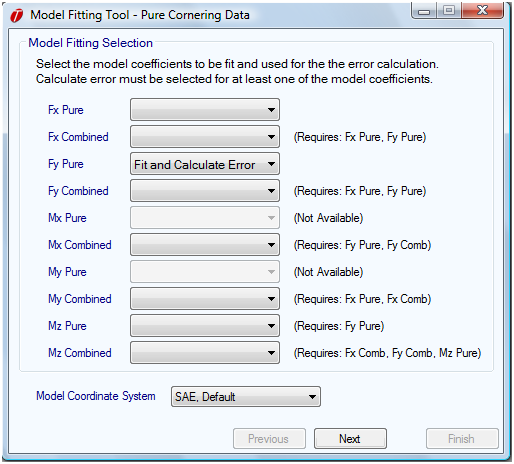
\includegraphics[width=1.0\textwidth]{ModelFittingRequirements.png}
	\caption{Model Fitting Requirements}
	\label{fig:ModelFittingRequirements}
\end{figure}

The two most common model fitting sequences will be described in Table~\ref{tbl:ModelFittingOrder} and Table~\ref{tbl:ModelFittingOrder2}. The first sequence uses pure lateral and combined data like the model fitting example in the previous sections. The second sequence uses pure lateral, pure longitudinal and combined data.
Under \textsl{Coefficients to be Fixed} the "Fix" indicates that these coefficients should be selected in the Advanced Fitting Options window. Under Coefficients to be Fit the "FE" indicates that these coefficients should be set to \textsl{Fit and Calculate Error} and the "Fit" indicates that these coefficients should be set to \textsl{Fit} in the \textsl{Model Fitting Selection} window.

\begin{table} [H]
	\centering
			\begin{tabular}{|c|c|c|c|c|c|c|c|c|c|c|c|c|c|}
			\hline
			\multicolumn{14}{|c|}{\cellcolor{tblue}\textbf{Model Fitting with Pure Lateral and Combined Data}} \\ \hline
			\multirow{3}{*}{Step} & \multirow{3}{*}{Data Used} & \multicolumn{6}{|c|}{\cellcolor{ttblue}Coefficients to be Fixed} & \multicolumn{6}{|c|}{\cellcolor{ttblue}Coefficients to be Fit} \\ \cline{3-14}
			 & &\multicolumn{3}{|c|}{Pure}&\multicolumn{3}{|c|}{Combined}&\multicolumn{3}{|c|}{Pure}&\multicolumn{3}{|c|}{Combined} \\ \cline{3-14}
			 & &Fx	&Fy	&Mz	&Fx	&Fy	&Mz	&Fx	&Fy	&Mz	&Fx	&Fy	&Mz \\ \hline
			 1 & Pure Lat. & & & & & & & &Fe& & & & \\ \hline
			 2 & Pure Lat. & & Fix& & & & & &&Fe & & & \\ \hline
			 5 & Combined. & & Fix&Fix & & & &Fit  & & &Fe & & \\ \hline
			 4 & Combined. &Fix & Fix&Fix &Fix & & & & & & &Fe & \\ \hline
			 5 & Combined. &Fix & Fix&Fix &Fix &Fix & & & & & & &Fe \\ \hline
		\end{tabular}
	\caption{Model Fitting Order with Pure Lateral and Combined Data}
	\label{tbl:ModelFittingOrder}
\end{table}

\begin{table} [H]
	\centering
			\begin{tabular}{|c|c|c|c|c|c|c|c|c|c|c|c|c|c|}
			\hline
			\multicolumn{14}{|c|}{\cellcolor{tblue}\textbf{Model Fitting with Pure Lateral, Pure Longitudinal and Combined Data}} \\ \hline
			\multirow{3}{*}{Step} & \multirow{3}{*}{Data Used} & \multicolumn{6}{|c|}{\cellcolor{ttblue}Coefficients to be Fixed} & \multicolumn{6}{|c|}{\cellcolor{ttblue}Coefficients to be Fit} \\ \cline{3-14}
			 & &\multicolumn{3}{|c|}{Pure}&\multicolumn{3}{|c|}{Combined}&\multicolumn{3}{|c|}{Pure}&\multicolumn{3}{|c|}{Combined} \\ \cline{3-14}
			 & &Fx	&Fy	&Mz	&Fx	&Fy	&Mz	&Fx	&Fy	&Mz	&Fx	&Fy	&Mz \\ \hline
			 1 & Pure Lat. & & & & & & & &Fe& & & & \\ \hline
			 2 & Pure Lat. & & Fix& & & & & &&Fe & & & \\ \hline
			 5 & Combined. & & Fix&Fix & & & &Fit  & & &Fe & & \\ \hline
			 4 & Combined. &Fix & Fix&Fix & & & & & & & & & \\ \hline
			 5 & Combined. &Fix & Fix&Fix &Fix & & & & & & & & \\ \hline
			 6 & Combined. &Fix & Fix&Fix &Fix &Fix & & & & & & & \\ \hline
		\end{tabular}
	\caption{Model Fitting Order with Pure Lateral, Pure Longitudinal and Combined Data}
	\label{tbl:ModelFittingOrder2}
\end{table}

\section{Model Coefficient Form}
\label{sec:ModelCoefficientForm}
After a model is fit the coefficients corresponding to it can be accessed by clicking on the model in the tire project tree. This will display the model coefficient form in the data entry area as shown in Figure~\ref{fig:ModelCoefficientForm}. This form includes the model coefficients, a description box, and the option to change the name displayed in the legend for the model. In this form the model coefficients can be modified by the user. This will be covered in detail in the next section. 

\begin{figure}[H]
	\centering
		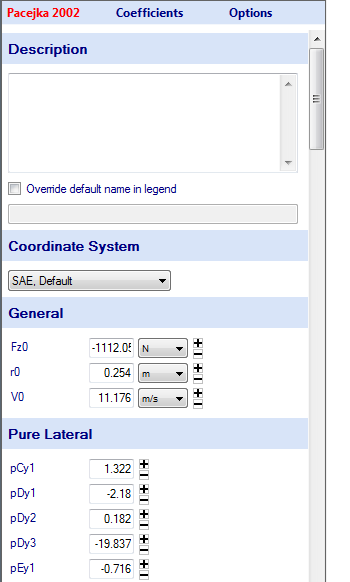
\includegraphics[height=0.6\textheight]{ModelCoefficientForm.png}
	\caption{Model Coefficient Form}
	\label{fig:ModelCoefficientForm}
\end{figure}

After a model is fit information regarding the model fitting will be directly imported into the description box as can be seen in Figure   The information included in the description box is the final error of the fitting, the model that was fit, the data file used, the coefficients fit, the error evaluation method, the coefficient boundary, and the solver parameters.

\section{Adjusting Models}
\label{sec:AdjustingModels}
Once the model is created and graphed against the raw data you might want to adjust it to improve its accuracy in a certain region or improve its behavior beyond the measurement area.  This can be done easily in OptimumTire.
  
Selecting a tire model in the project tree will show the model coefficients in the data entry area. You can modify the coefficients by 10\% by double clicking on the "+" or "-" button next to the coefficient \footnote[1]{When clicking the "+" and "-" button, the coefficient is either  multiplied or divided 1.10} . If the model is shown on a graph (see chapter~\ref{sec:AdditionalFeatures} for information about graphing), holding down the "+" or "-" button will show a preview of the model with the coefficient modified by 10\%. An example of this is shown in Figure~\ref{fig:ModelAdjustment}. In this figure the "+" button of the $pDy1$ coefficient is being held down. As can be seen in Figure~\ref{fig:ModelAdjustment} this change has a large effect on the graph. Changing other coefficients will have a much different effect on the curve both in terms of its magnitude and shape. The coefficients can also be adjusted manually by changing the values in the boxes. When applied to a tire model the coefficients of a scaling factor can be adjusted in the same way.

\begin{figure}[H]
	\centering
		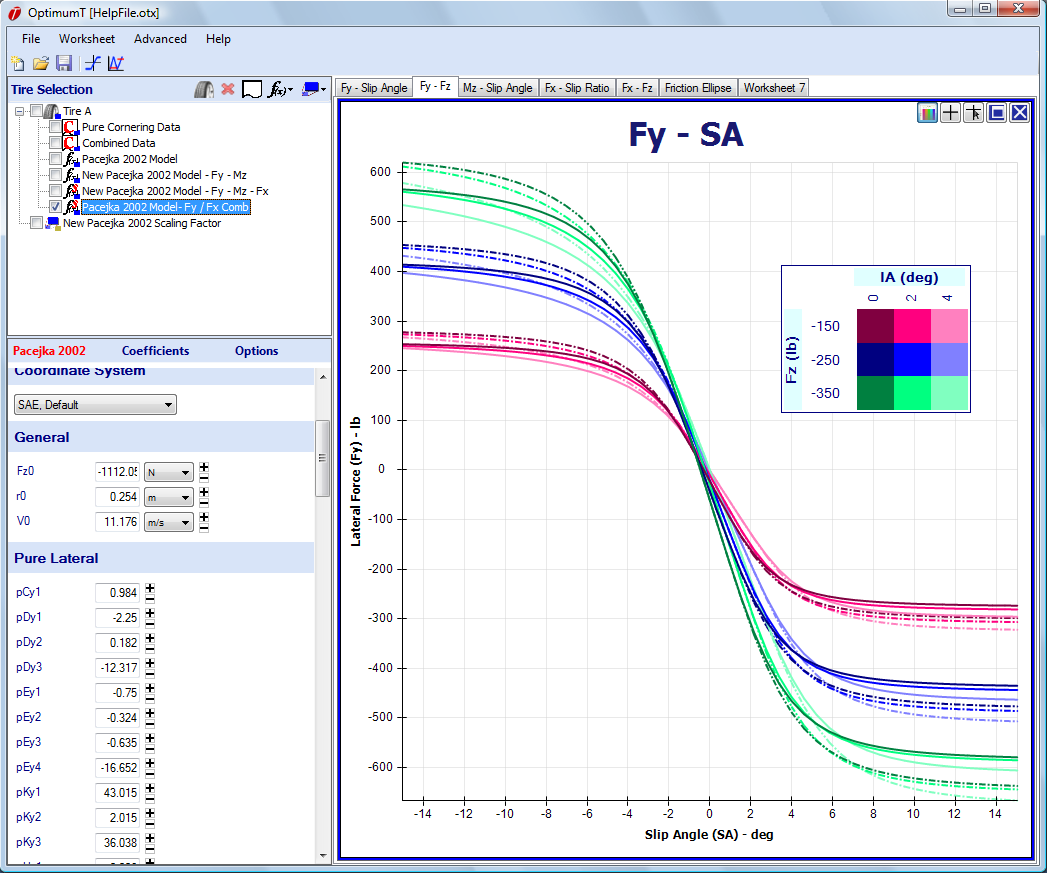
\includegraphics[width=1.0\textwidth]{ModelAdjustment.png}
	\caption{Model Adjustment Preview Feature}
	\label{fig:ModelAdjustment}
\end{figure}


\section{Creating Coefficient Boundaries From an Existing Model}
\label{sec:boundaryFromModel}

You can create a boundary from an existing model. When doing this, you specify the half-width of the boundary. In the model coefficient form, click on \textit{Options} then \textit{Create Boundary From Model} to arrive at the range specification (shown in Figure \ref{fig:BoundaryFromModel}). Enter the desired range and click the check-mark button. The minimum for each coefficient is created by reducing the the coefficient value by the user specified percentage, and the maximum is created by increasing the the value by the same amount. For example, if one of the coefficients of the model has a value or $1.00$ and you specify a boundary range of $10\%$, the minimum will be $0.90$ and the maximum will be $1.10$.

\begin{figure}
	\centering
		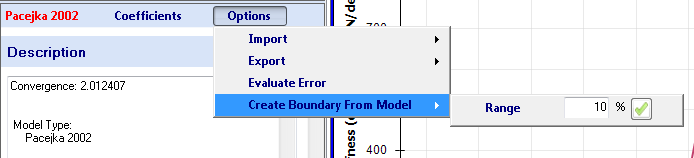
\includegraphics[width=0.80\textwidth]{BoundaryFromModel.png}
	\caption{Creating a boundary from an existing model.}
	\label{fig:BoundaryFromModel}
\end{figure}

Once you have clicked the check-mark button to create the boundary, you will be presented with the dialog shown in Figure \ref{fig:BoundaryFromModelSaveAs}. Enter the name to save the boundary as and choose a folder to put the boundary in.

\begin{figure}
	\centering
		\includegraphics[width=0.40\textwidth]{BoundaryFromModelSaveAs.png}
	\caption{To save the boundary created from a model, specify the name to save it as in this dialog.}
	\label{fig:BoundaryFromModelSaveAs}
\end{figure}

\include{graphing}
\chapter{Custom Models}

\setcounter{figure}{0}
\setcounter{table}{0}

\label{sec:CustomModels}

\section{Introduction to Custom Models}
\label{sec:IntroductiontoCustomModels}

Custom models are part of the advanced features available in OptimumTire. This fucntionality gives users the flexibility to include user developed custom models within the OptimumTire environment. With the custom models feature users can write their own models in house, therefore keeping proprietary models confidential and providing the ability to tailor models to the exact specifications required. Custom models need only to be coded once, they can then be used repeatedly and as efficiently as any of the hard coded models available within OptimumTire.
The custom model package is an advanced feature which requires an additional activation license available by contacting ~\href{mailto: engineering@optimumg.com}{engineering@optimumg.com}\\

\section{Creating Custom Models}
\label{sec:CreatingCustomModels}
Custom models are based on a template written in C\# this template is provided by OptimumG with the purchase of the custom models package. To create a new model the user must first define a .dll (dynamically linked library) file which can then be loaded into OptimumTire. This file references the template provided by OptimumG so it must follow a certain syntax that makes it compatible with OptimumTire. This syntax is outlined in Sections~\ref{sec:CreatingaCoefficientFile} and ~\ref{sec:CreatingaCalculationFile}. The user .dll contains a list of coefficients and equations that define the user's custom model.

An example project is included with OptimumTire to provide an example that users can copy and edit when developing custom models. The project is installed in My Documents on the users machine and can be opened with Visual C\#.

\subsection{Software Requirements}
\label{sec:CustomModelsSoftwareRequirements}

The custom model template is written in Visual C\# a CLI (Common Language Infrastructure) language. In order to create a custom model the user must first download a version of Visual C\# by Microsoft. This software is available as a free \textsl{Express Edition} for the general user or \textsl{Visual Studio Professional Edition} for professional software developers. For the purposes of creating OptimumTire custom models the \textsl{Visual C\# Express Edition} is sufficient. The download is availble at the following site ~\href{http://www.microsoft.com/express/Downloads/#2010-Visual-CS}{www.microsoft.com/express/Downloads}

OptimumTire requires two files a \textsl{Coefficient File} and a \textsl{Calculation File} to define a model. The follwing sections outline how to create these files.

\subsection{Creating the Custom Model Project}
The first step in creating custom model is to create a new C\# project with the coefficient and calculation classes. To do this open Visual Studio or Visual C\#. Create a new model from the file menu, select \textsl{C\# Class Library} and enter the name of your model as shown.

 \begin{figure}[H]
	\centering
		\includegraphics[width=1.0\textwidth]{NewCustomModelProject.png}
	\caption{Creating a New Project}
	\label{fig:CreatingaNewProject}
\end{figure}

Alternatively you can open the example project provided with OptimumTire, modify it and save it under a different name.

Next right click on the project just created and select add->new item to add a class to the project.

 \begin{figure}[H]
	\centering
		\includegraphics[width=1.0\textwidth]{NewCustomModelClass.png}
	\caption{Creating a New Class}
	\label{fig:CreatingaNewClass}
\end{figure}

Add two classes, the coefficient class and the calculation class. Name these classes \textsl{CustomTireModelCoef} and \textsl{CustomTireModelCalculation}. Save the project and then continue with the following steps.

\subsection{Referencing the Custom Model Template}
\label{sec:ReferencingtheCustomModelTemplate}

Once the project has been created the next step is to add the reference for the custom model template. Without this reference the custom model classes defined by the user cannot inherit from the template.
To add a reference to a project first right click on the C\# project and select add reference from the dropdown menu as shown in Figure~\ref{fig:CreatingaReference}.

 \begin{figure}[H]
	\centering
		\includegraphics[height=0.3\textheight]{creatingReference.png}
	\caption{Creating a Reference}
	\label{fig:CreatingaReference}
\end{figure}

Select the browse tab in the add reference dialog and browse to the OptimumTire installation folder. Select the CustomTireModelTemplate.dll and select OK as shown in Figure~\ref{fig:SelectingtheReferencedll}. The reference to the template.dll should now appear in the project references folder in the Visual Studio Solution Explorer. 

 \begin{figure}[H]
	\centering
		\includegraphics[height=0.4\textheight]{SelectTemplate.png}
	\caption{Selecting the Reference .dll}
	\label{fig:SelectingtheReferencedll}
\end{figure}

\subsection{Creating a Coefficient File}
\label{sec:CreatingaCoefficientFile}

An example coefficient file has been included with the OptimumTire custom package. It is shown in Figure~\ref{fig:CoefFileVC}. It has a number of features. 

 \begin{figure}[H]
	\centering
		\includegraphics[width=1.0\textwidth]{CoefFileVC.png}
	\caption{Visual C\# Coefficient File}
	\label{fig:CoefFileVC}
\end{figure}

The first section is the \textsl{\textquotedbl Namespace Declaration\textquotedbl} this is the name of the custom .dll file and will be used as an identifier within OptimumTire.

The second statement is the \textsl{\textquotedbl Inheritance Statement\textquotedbl}. This is required to ensure all the template functions are available to the custom .dll. Without this statement the .dll will produce an error when loaded into OptimumTire. The coefficient file must inherit from the coefficient template CustomTireModelTemplate.TireModelCoef.

The third statement is the \textsl{\textquotedbl Model Description\textquotedbl} which will appear in the description box on the model coefficient form sheet.

The fourth section contains the \textsl{\textquotedbl Coefficient Definitions\textquotedbl} themselves. It is a list of the coefficients to be added to the array list. These statements are in the format shown at the start of this section.

The fifth section is the \textsl{\textquotedbl Function Requirements\textquotedbl}. These statements allow the user to change the function dependencies in the model. For example the aligning moment function often requires the the lateral force to be calculated frist. Therefore the function requirement for \textsl{CalculateMz} will be \textsl{FunctionMask.FunctionFy}. The function requirements statements are in the following syntax.

\textbf{\texttt{m\_MzPureReq = (int)(FunctionMask.FunctionFy);}}

setting a function requirement equal to -1 will make that function unavailable. Setting the requirement equal to 0 indicates that the function does not have any dependencies.

The coefficient file is simply an arraylist of coefficients. Each coefficient is defined in the following format:

\texttt{\textbf{newCoefficient((\textquotedbl Name\textquotedbl , Default Value, Function Mask, Coordinate System Definition, Constraint Boolean)}}

\begin{itemize}
\item	\textbf{Name:} The name of the variable that will appear beside each variable in OptimumTire.  Must be entered as a string enclosed in quotation marks \textquotedbl \textquotedbl
\item	\textbf{Default Value:} The default value of the coefficient that will apear when creating empty models, boundary files and constraints. This value is a single floating point number.
\item \textbf{Function Mask:} Tells OptimumTire which outputs are related to each coefficient so the solver knows which coefficients to fit when fitting a specific model. OptimumTire has a list of function masks to choose from:


\begin{center}

\texttt{\textbf{FunctionMask.FunctionFx \\
FunctionMask.FunctionFy \\
FunctionMask.FunctionFz \\
FunctionMask.FunctionMx \\
FunctionMask.FunctionMy \\
FunctionMask.FunctionMz \\
FunctionMask.FunctionRl \\
FunctionMask.FunctionScale}}
\end{center}

Each coefficient must include one of these definition or a combination of the above separated by the or \textquotedbl | \textquotedbl operator. 

For example a coefficient \textsl{\textquotedbl U\textquotedbl} is used in the equations for calculating the lateral force, longitudinal force and aligning torque its coefficient mask is therefore:

\texttt{\textbf{FunctionMask.FunctionFx | FunctionMask.FunctionFy | FunctionMask.FunctionMz}}

The function mask FunctionScale is used to specify that the coefficient is used as a scaling factor(see Section~\ref{sec:ModelScalingFactors}). This means the coefficient will not be fit in the fitting proccess and will remain the default value specified. The default value should be 1.0 in most cases for the scaling factors to have no effect on the model.

\item \textbf{Coordinate System Definition:} The coordinate properties of the coefficient that determine which coordinate system conversion will cause the coefficient to change sign. Each coordinate system definition is in the form CSDfn.X which means, that if the sign of the input X changes in a coordinate system  conversion the coefficients with the corresponding coordinate system definition will also change sign. OptimumTire provides the following coordinate system definitions:
 	
\begin{center}

\texttt{\textbf{   	CSDefn.V \\
    CSDefn.SA \\
    CSDefn.SR \\
    CSDefn.IA \\
    CSDefn.F~\_x \\
    CSDefn.F~\_y \\
    CSDefn.F~\_z \\
    CSDefn.M~\_x \\
    CSDefn.M~\_y \\
    CSDefn.M~\_z \\
    CSDefn.None}}
\end{center}

Note: Leaving the coordinate system definition as \textsl{CSDefn.None} means the coefficient will not be affected by any coordinate system conversions within OptimumTire so the coefficients will always remain in the initially selected system.

OptimumTire supports four coordinate systems these are the SAE, Adapted SAE, ISO and Adapted ISO coordinate systems. For definitions of these systems see Section~\ref{sec:CoordinateSystems}. These coordinate systems will apply the following coordinate system changes when converting from the default SAE coordinate system:

        \textbf{SAE:} {\tt Default} \\
        \textbf{Adapted SAE:}  {\tt CSDefn.SA | CSDefn.F\_z} \\
        \textbf{ISO:} {\tt CSDefn.SA | CSDefn.F\_y | CSDefn.F\_z | CSDefn.M\_y | CSDefn.M\_z} \\
        \textbf{Adapted ISo:} {\tt CSDefn.IA | CSDefn.F\_y | CSDefn.F\_z | CSDefn.M\_y | CSDefn.M\_z}

\item \textbf{Constraint Boolean:} Defines whether a coefficient will be a fixed constraint or not. True if coefficient of fixed or false if it is a coefficient is to be fit.
\end{itemize}

\subsection{Creating a Calculation File}
\label{sec:CreatingaCalculationFile}

The calculation file contains the equations that define the tire model. An example of how to create a calculation file is included with the OptimumTire custom model package. The example is shown in Figure~\ref{fig:CalcFileVC}.

 \begin{figure}[H]
	\centering
		\includegraphics[width=1.0\textwidth]{CalcFileVC.png}
	\caption{Visual C\# Calculation File}
	\label{fig:CalcFileVC}
\end{figure}

The file contains several statements. The first is the \textsl{\textquotedbl Namespace Declaration\textquotedbl} this is the name of the .dll and will be used by OptimumTire as an identifier for the custom model. It must be the same as the \textsl{\textquotedbl Namespace Declaration\textquotedbl} in the coefficient file.

The second statement is the \textsl{\textquotedbl Inheritance Statement\textquotedbl}. This is required to ensure all the template functions are available to the custom .dll. Without this statement the .dll will produce an error when loaded into OptimumTire. The coefficient file must inherit from the calculation template CustomTireModelTemplate.TireModelCalculation.

The third section contains the function definitons themselves. The primary functions must be declared in the following format to override the fucntions in the template file.

\texttt{\textbf{public override float CalculateXXXXX(float Fz, float SA, float SR, float IA, float V, float P, ref CustomTireModelTemplate.TireModelCoef coef)}}

The custom calculation template contains the following overridable functions that can be redefined by the user.

\begin{center}
\texttt{\textbf{CalculateFxPure(Fz, SA, SR, IA, V, P, ref coef)\\
	        CalculateFxComb(Fz, SA, SR, IA, V, P, ref coef)\\
	        CalculateFyPure(Fz, SA, SR, IA, V, P, ref coef)\\
	        CalculateFyComb(Fz, SA, SR, IA, V, P, ref coef)\\
	        CalculateMxPure(Fz, SA, SR, IA, V, P, ref coef)\\
	        CalculateMxComb(Fz, SA, SR, IA, V, P, ref coef)\\
	        CalculateMyPure(Fz, SA, SR, IA, V, P, ref coef)\\
	        CalculateMyComb(Fz, SA, SR, IA, V, P, ref coef)\\
	        CalculateMzPure(Fz, SA, SR, IA, V, P, ref coef)\\
	        CalculateMzComb(Fz, SA, SR, IA, V, P, ref coef)\\
	        CalculateLoadedRadius(Fz, SA, SR, IA, V, P, ref coef)}}
\end{center}

    
These functions define the primary outputs of OptimumTire. The user may include any number of additional functions that may be called from within these primary functions. It should be noted that the quality of the code in the calculation file will affect the speed of the fitting and graphing processes.
Each function must follow the signature of the functions defined in the template file. Each function returns a single floating point value for the input values Fz, SA, SR, IA, V, P and the coefficient array.

When writing the functions themselves the user can refer to the coefficients by their name as previously defined in the coefficient file. eg. {\tt coef[\textquotedbl A0 \textquotedbl]}. 

\subsection{Common Programming Errors}
\label{sec:Common Programming Errors}
The following are common errors made when programming in C\#. Check the following basic syntax before compiling your custom .dll.

\begin{itemize}
	\item In C\# each command should be placed on a new line which ends with the \textquotedbl ;\textquotedbl character.

\item Functions, classes, loops and conditional statements are defined by braces. Each \textquotedbl \{\textquotedbl must have a matching  \textquotedbl \}\textquotedbl.

\item Each function must have the correct signature. Use intellisense to make sure that each function passes all the required parameters.
\end{itemize}

For more information on programming in C\# see ~\href{http://www.msdn.com}{www.msdn.com}

\section{Importing Custom Models in OptimumTire}
\label{sec:ImportingCustomModelsinOptimumTire}

Once the user has created or been given a custom model .dll file it can be loaded into OptimumTire. To load the custom model select the \textsl{Advanced} menu item in OptimumTire then selct the \textsl{Custom Tire Model} item from the dropdown menu as shown in Figure~\ref{fig:AdvancedFeaturesMenu}.

\begin{figure}[H]
	\centering
		\includegraphics{AdvancedCustomTireModel.png}
	\caption{Advanced Features Menu}
	\label{fig:AdvancedFeaturesMenu}
\end{figure}

Selecting the \textsl{Custom Tire Model} item will launch the \textsl{Custom Tire Model Manager} shown in Figure~\ref{fig:CustomTireModelManager}.

 \begin{figure}[H]
	\centering
		\includegraphics{CustomTireModelManager.png}
	\caption{Custom Tire Model Manager}
	\label{fig:CustomTireModelManager}
\end{figure}

The \textsl{Custom Tire Model Manager} shows the list of custom models currently available in OptimumTire. The user can add or delete models from the list using the add and delete buttons. Note that OptimumTire uses the name of the .dll as an identifier so two custom models cannot be added with the same name. See sections~\ref{sec:CreatingaCoefficientFile} and ~\ref{sec:CreatingaCalculationFile} for how to name custom models.

Clicking on the \textsl{Add} button opens a standard windows dialog. Navigate to the location of the custom .dll that is to be added and click \textsl{OK} to add the model to the list.

\section{The Custom Model Fitting Process}
\label{sec:The CustomModelFittingProcess}

To fit a custom model the user can follow the same process used for standard model fitting. The \textsl{Custom Model} option should appear at the bottom of the list of models available to fit in the model fitting dropdown menu as shown in Figure~\ref{fig:CustomModelFitting}.

 \begin{figure}[H]
	\centering
		\includegraphics{CustomFitting.png}
	\caption{Custom Model Fitting}
	\label{fig:CustomModelFitting}
\end{figure}

Selecting the \textsl{Custom Model} item from the dropdown will bring up the \textsl{Custom Model Selection Dialog} shown in Figure~\ref{fig:CustomTireModelSelection}. Select the custom model to be fit by either double clicking on it, or selecting it and clicking the \textsl{OK} button. This will launch the fitting process.

The main differences in the custom fitting process are the constraints and boundary files. Which coefficients appear in the \textsl{Constraints Wizard} will depend on the \textsl{Constraint Boolean} specified in the coefficient file created by the user (see Section~\ref{sec:CreatingaCoefficientFile}). Also the boundaries wizard will not contain predefined templates so a new boundary must be created for each new custom model.

 \begin{figure}[H]
	\centering
		\includegraphics{CustomModelSelection.png}
	\caption{Custom Tire Model Selection}
	\label{fig:CustomTireModelSelection}
\end{figure}

\section{Custom Model Import and Export}
\label{sec:CustomModelImportandExport}

The import and export functions work for the custom model in the same way as the standard tire models in OptimumTire (see Section~\ref{sec:ImportandExportModels}).

However to export models to .tir or Excel format the user must first create a template for each model. The process for creating and modifying export templates is illustrated in Section~\ref{sec:ImportandExportModelsExportTemplate}. %moketag uncomment this when the custom models package is ready to be released

\chapter{Additional Features}
\setcounter{figure}{0}
\setcounter{table}{0}

\label{sec:AdditionalFeatures}
\section{OptimumTire Add-in}
\label{sec:OptimumTAddin}

The OptimumTire add-in allows users to access all of the output quantities in OptimumTire from Excel, Matlab or any other software package that supports COM components. Simulations and calculations that require a tire model can be done easily using this feature. Look-up tables of the tire charactereistics can also be created quickly for use in other applications. 

In the add-in, the model coefficients are specified to the OptimumTire functions with long character strings. These strings can be directly exported from OptimumTire. To do this first click on the desired tire model in the project tree. This will expose the model coefficients in the data entry area. Then click on the \textit{Options} button as shown in Figure~\ref{fig:AddinExport}. Then select \textit{Export} and \textit{Add-in Model to Clipboard}. This will copy the encoded string to the computer clipboard and allow it to be pasted into Excel or any other software.

\begin{figure}[H]
	\centering
		\includegraphics[width=1.0\textwidth]{AddinExport.png}
	\caption{Export the Encoded Model Coefficients from OptimumTire}
	\label{fig:AddinExport}
\end{figure}

The inputs and outputs of the add-in are expected to be in the coordinate system defined for the model. The syntax used for the inputs of the functions is demonstrated in the following equation.

\begin{center}
\texttt{Output = Function(Fz, SA, SR, IA, V, P, ModelCoefficients)}
\end{center}

The coordinate system can be queried using the command:
\begin{center}
\texttt{GetModelInfo(ModelCoefficients)}
\end{center}

The units used are also restricted. The units used are displayed in Table~\ref{tbl:AddinUnits}. The values calculated are outputted in the same units as those in the table.

\begin{center}
\begin{longtable}{|c|c|}
			
			\hline
			\multicolumn{2}{|c|}{\cellcolor{tblue}\textbf{Add-in Units}} \\ \hline
			\rowcolor{ttblue}\textbf{Inputs} & \textbf{Unit} \\ \hline
			Normal Load (Fz) &Newton \\ \hline
			Inclination Angle (IA)	&degree \\ \hline
			Slip Angle (SA)	&degree \\ \hline
			Slip Ratio (SR)	&ratio \\ \hline
			Speed (V)	&meter/sec \\ \hline
			Pressure (P)	&bar \\ \hline
			\hline
											
			\caption{Units used in the OptimumTire Add-in}
			\label{tbl:AddinUnits}
			
\end{longtable}
\end{center}

\subsection{Using the Add-in with Excel}
\label{sec:OptimumTAddin:Excel}

The installation and use of the add-in in Excel 2007 will be demonstrated. Once OptimumTire is installed the Add-in can be accessed easily from Excel. First the user should click the \textit{Start} button in the top left corner of Excel. Then click the \textit{Excel Options} button as shown in Figure~\ref{fig:ExcelOptions}.

\begin{figure}[H]
	\centering
		\includegraphics[width=.75\textwidth]{ExcelOptions.png}
	\caption{Excel Options}
	\label{fig:ExcelOptions}
\end{figure}

Once the Excel options are open click on \textit{Add-Ins} on the left side of the window. In the dropdown box labeled \textit{Manage:} near the bottom of the window select \textit{Excel Add-ins}. This is shown in Figure~\ref{fig:ExcelAddins} Then click on the \textit{Go} button. 

\begin{figure}[H]
	\centering
		\includegraphics[width=1.0\textwidth]{ExcelAddins.png}
	\caption{Excel Add-Ins}
	\label{fig:ExcelAddins}
\end{figure}

\begin{figure}[H]
	\centering
		\includegraphics[width=.4\textwidth]{ImplementingAddin.png}
	\caption{Implementing the OptimumTire Add-In}
	\label{fig:ImplementingAddin}
\end{figure}


The \textit{Add-ins} selection window will now appear. In Figure~\ref{fig:ImplementingAddin} \textit{OptimumT.Calculations} is shown in the list of add-ins. This add-in will have to be added to list by clicking on the button labeled \textit{Automation...}. This will open the \textit{Automation Server} window as shown in Figure~\ref{fig:AutomationServer}. Selecting \textit{OptimumT.Calculations} and pressing the \textit{OK} button will load the COM add-in into Excel. Now the add-in can be used in the same way as functions built into Excel.

\begin{figure}[H]
	\centering
		\includegraphics[width=.9\textwidth]{AutomationServer.png}
	\caption{Selecting the COM Add-in in Excel }
	\label{fig:AutomationServer}
\end{figure}


Now the Add-in can be used in Excel by clicking on the \textit{Insert Function} button in Excel. This will open the window shown below in Figure~\ref{fig:InsertFunction}. The available functions will be displayed by selecting \textit{OptimumTExcelAddin} in the categories dropdown box.

\begin{figure}[H]
	\centering
		\includegraphics[width=.8\textwidth]{InsertFunction.png}
	\caption{Inserting OptimumTire Functions into Excel}
	\label{fig:InsertFunction}
\end{figure}

Then the parameters of the function can be inputted as shown in Figure~\ref{fig:AddinResults}. As can be seen in this figure the input parameters are the six tire model inputs (normal load, slip angle, slip ratio, inclination angle, velocity and inflation pressure) and the tire model coefficients. The tire model coefficients are inputted as an encoded string as shown in Figure~\ref{fig:AddinEncodedCoefficient}.

\begin{figure}[H]
	\centering
		\includegraphics[width=1.0\textwidth]{AddinResults.png}
	\caption{OptimumTire Add-in Input Parameters}
	\label{fig:AddinResults}
\end{figure}

\begin{figure}[H]
	\centering
		\includegraphics[width=1.0\textwidth]{AddinEncodedCoefficient.png}
	\caption{Encoded String that represents the Model Coefficients}
	\label{fig:AddinEncodedCoefficient}
\end{figure}


\subsection{Matlab COM Add-in}
\label{sec:OptimumTAddin:COMMatlab}

The use of the COM add-in in Matlab is demonstrated in this section. Every time that Matlab is opened the add-in needs to be loaded. The add-in is loaded in Matlab using the \textit{actxserver} function as shown below in Figure~\ref{fig:MatlabAddin}. Then all of the add-in functions can be accessed through the \textit{handle.method} syntax, were \textit{handle} is the variable that the add-in was loaded as and \textit{method} is the OptimumTire function that is to be used. In the figure below \textit{example} is the handle and \textit{GetLicense}, \textit{CalculateFy} and \textit{CalculateCorneringStiffness} are all functions. To get the full list of the available functions just type \textit{handle.Methods} in the Matlab command window.

\begin{figure}[H]
	\centering
		\includegraphics[width=1.0\textwidth]{MatlabAddin.png}
	\caption{Using the OptimumTire Add-in in Matlab}
	\label{fig:MatlabAddin}
\end{figure}

An example of the add-in being used in a m-file is shown in Figure~\ref{fig:mfileAddin}. In this example the handle variable(h in this case) is checked to see if it exists. If it does not exist then it loads the add-in. If it does already exist the add-in is not reloaded. This Matlab m-file is also included with OptimumTire. It is located in the \textit{Documents} folder of the user who installed OptimumTire in a folder called \textit{Matlab COM Addin}.

\begin{figure}[H]
	\centering
		\includegraphics[width=1.0\textwidth]{mfileAddin.png}
	\caption{Using the OptimumTire Add-in in a Matlab m-file}
	\label{fig:mfileAddin}
\end{figure}

\subsection{Using the COM Addin in Programs}
\label{sec:OptimumTAddin:ComProgram}

The exact method for using the OptimumTire add-in with your own programs will depend on your programming environment. Please refer to the documentation that supplied with your programming environment for details on using COM components.

In most environments, you will need to add a reference to the OptimumTire type library. This is called \texttt{OptimumT 1.0 Type Library} or \texttt{OptimumTLib}.

There is an example C\# project provided with OptimumTire. It is located in the \textit{Documents} folder of the user who installed OptimumTire in a folder called \textit{OptimumTAddinExample}. The main function for this program is:


\begin{verbatim}
static void Main(string[] args)
{

    Console.WriteLine("Welcome to the OptimumTire Add-in example program\n\n");
           
    string modelCoef = "CAAAAAAAGHAAAAAAAAPELJFMGGGGGKODAAAAAKBEAJGPMLPDA" +
        "JJIEFPLNLHAAAODEGJIGBAMFAOJCLPLOLKEMCNLBODPFNNLKNOLOEODEF" +
        "BFFFBEJBLJCLPDHLONLLMDKFOAJHKDPGDCEELLNIHNCOMLODBJIJLLCMD" +
        "NJANDAKBPFDPLGJNNGIPLIMNKOJPDICBKMHPDEJDNMMNLGAODMDAMNELK" +
        "NMNDFJJCPJLDLNEJGILLNMHPLIBMDMNBAOBEOFBKBLPDLPFNCKILEHLCC" +
        "JKDNIBOCJIDBPNDMILDPDGNMABEDPBOJOAMMFEBCJPDOIFECOKDDMPDCO" +
        "MDCHNCOIOLKKJGMEBEFCJCBCBEMIMFMFLDFAGGKHPDMGNFBGMDMDANLHM" +
        "DKPIHEKKLABLCAEODKNGEIIAEJHMKKBAEBGKBANOLOHEJBDCMHFOFEJPL" +
        "KFAGCFMLAAAAAAAAAAAAAAAAAAAAAAAAAAAAAAAAAAAAAAAAAAAAAAAAA" +
        "AAAAAAAAAAAAAAAAAAAAAAAAAAAAAAAAAAAAAAAAAAAAAAAAAAAAAAAAA" +
        "AAAAAAAAAAAAAAAAAAAAAAAAAAAAAAAAAAAAAAAAAAAAAAAAAAAAAAAAA" +
        "AAAAAAAAAAAAAAAAAAAAAAAAAAAAAAAAAAAAAAAAAAAAAAAAAAAAAAAAA" +
        "AAAAAAAAAAAAAAAAAAAAAAAAAAAAAAAAAAAAAAAAAAAAAAAAAAAAAAAAA" +
        "AAAAAAAAAAAAAAAAAAAAAAAAAAAAAAAAIPDAAAAAIPDAAAAAIPDAAAAAA" +
        "AAAAAAAIPDAAAAAIPDAAAAAIPDAAAAAIPDAAAAAIPDAAAAAIPDAAAAAIP" +
        "DAAAAAIPDAAAAAIPDAAAAAIPDAAAAAIPDAAAAAIPDAAAAAIPDAAAAAIPD" +
        "AAAAAIPDAAAAAIPDAAAAAIPDAAAAAIPDAAAAAIPDAAAAAIPDAAAAAIPD";

    OptimumTLib.Calculations calc = new OptimumTLib.Calculations();

    // Display the type of model and the coordinate system
    Console.WriteLine("The model is:");
    Console.WriteLine(calc.GetModelInfo(modelCoef));


    // set up variables to plug into the tire model
    float Fz = -3000.0f;    // the vertical load [N]
    float IA = 1.0f;        // the inclination angle [deg]
    float SR = 0.0f;        // the slip ratio [fraction]
    float V = 10;           // the speed [m/s]
    float P = 2;            // the inflation pressure [bar]

    // declare a variable to store the calculated lateral force in
    float Fy;
            
    Console.Write("\n\n   SA      Fy\n");
    // loop through a series of slip angles and display the resulting force
    for (float SA = -10.0f; SA <= 10.0f; SA+=2.0f)
    {
        Fy = calc.CalculateFy(Fz, SA, SR, IA, V, P, modelCoef);
        Console.WriteLine(string.Format("{0,5} {1,10}", SA, Fy));
    }

    Console.Write("\nPress any key to exit...");
    Console.ReadKey();
}
\end{verbatim}

			
\section{Template Manager}
\label{sec:TemplateManager}

The template manager allows the user to easily organize or delete templates in OptimumTire. The template manager can be accessed by clicking on \textsl{Advanced} in the main toolbar and then clicking on \textsl{Template Manager}. A window similar to that shown in Figure~\ref{fig:TemplateManager} will open. In this window the user can manage graph templates, CSV import templates, coefficient boundaries and model export templates by clicking on the associated tabs. As can be seen in the figure the coefficient boundaries are organized by the different models. The models can be chosen from the dropdown box above the list of templates top of the window.

\begin{figure}[H]
	\centering
		\includegraphics[width=1.0\textwidth]{TemplateManager.png}
	\caption{Template Manager}
	\label{fig:TemplateManager}
\end{figure}

The templates can be deleted, renamed, or cloned using the buttons on the right side of the \textsl{Template Manager}. New folders can also be created so that the templates can be easily organized. The templates that are contained in the \textsl{Predefined} folder are included in OptimumTire and cannot be edited or deleted. However they can be cloned. When they are cloned the copied version of the template will be moved outside of the \textsl{Predefined} folder, so that it can be modified. The paste button allows the user to paste files from the clipboard into the appropriate folder which a useful feature when transfering large numbers of templates.

\section{Project Backups}
\label{sec:ProjectBackups}

OptimumTire saves a backup of the project before each save operation. This allows you to recover from a corrupted project or to recover if you accidentally made a unwanted change to the project and saved it. By default the last five revisions of the project are stored.

To go to a previous version of the project, click on the \textsl{Advanced} menu then on \textsl{Revert Project}. You will then see the \textsl{Revert Project} dialog (shown in Figure \ref{fig:RevertProject}). Select the backup that you wish to revert to and click on \textsl{Revert}. The date and time shown in this dialog is the time at which that version was initially created.

\begin{figure}[H]
	\centering
		\includegraphics[width=1.0\textwidth]{RevertProject.png}
	\caption{Revert Project dialog}
	\label{fig:RevertProject}
\end{figure}

When you revert a project, OptimumTire automatically creates a backup of the project immediately before reverting it. This allows you to "undo" a revert operation.

If a project fails to load, the \textsl{Revert Project} dialog will automatically be shown. This allows you to recover your project from an earlier backup.

\section{Error Evaluation}
\label{sec:ErrorEvaluation}

The \textsl{Error Evaluation} tool is shown in Figure~\ref{fig:ErrorEval}. This tool allows quick comparison of the error of the tire models against different sets of raw data. It also allows comparison between the four different types of error calculation. To access this tool first select the tire model for the error to be evaluate on in the project tree. At the top of the data entry form select \textsl{Options} and then \textsl{Evaluate Error}.

Once the \textsl{Error Evaluation} is open the data to be compared should first be selected in the list on the left. Then the models to base the error calculation should be selected. Clicking on the \textsl{Evaluate} button at the bottom of the window will calculate and display the error each of the different error calculation methods. 

\begin{figure}[H]
	\centering
		\includegraphics[width=1.0\textwidth]{ErrorEval.png}
	\caption{Error Evaluation}
	\label{fig:ErrorEval}
\end{figure}

\section{Lookup Table Export}
\label{sec:LookupTableExport}
OptimumTire offers the possibility to export lookup tables. These tables are compatible with simulation products such as CarSim or other software that uses a lookup table for modelling tyre performance rather than directly importing model coefficients and equations.
Lookup tables may be exported by selecting a model to export from the tree then clicking ~\textsl{Options->Export->Lookup table}. This will bring up the lookup table export form shown below.

\begin{figure}[H]
	\centering
		\includegraphics[width=1.0\textwidth]{LookupExportForm.png}
	\caption{Lookup Table Export Form}
	\label{fig:LookupExportForm}
\end{figure}

The form is split into three parts. The first is the \textsl{Page Tree}. Pages can be added to the export file by clicking the green \textsl{plus} sign and deleted by clicking the red \textsl{cross}. Pages may also be renamed in the tree, these names will provide the basis for the file names when exporting text files, or the sheet names when exporting to Excel. 

\begin{figure}[H]
	\centering
		\includegraphics[width=1.0\textwidth]{LookupExportFormPopulated.png}
	\caption{Lookup Table Export Settings}
	\label{fig:LookupExportFormPopulated}
\end{figure}

The second part of the form is the \textsl{Output Settings}. Each page in the page tree has an individual output settings sheet which specifies the parameters of the look up table. The output dropdown specifies which OptimumTire output will be used to populate the table. The \textsl{Vertical} and \textsl{Horizontal} dropdowns allow you to specify the type, range and step of the vertical and horizontal axes. The remaining boxes specify the values of the outputs to be held constant in the table.

The third part of the table is the \textsl{Format section}.  This specifies the global format for the export. Files may be exported as an MS Excel workbook or as text file. Text files may export multiple pages in one file or export each page to an individual file by selecting the \textsl{one page per file radio button}. When exporting files to excel a labels may be added to the tables to indicate the names of the table parameters. This is done by selecting the \textsl{Include Table Headings check box.} The text file delimiter may be adjusted using the delimiter drop down or a custom delimiter may be used by typing a delimiter in the \textsl{custom delimiter text box.}

A useful feature of the lookup table export is the ability to save the settings in a template for repeated exports. The \textsl{lookup table template bar} is located at the top of the form.  Templates may be applied using the dropdown menu or new templates saved using the save icons.

\chapter{Tips and Tricks}
\setcounter{figure}{0}
\setcounter{table}{0}

\label{sec:TipsandTricks}
\section{Plot All Data}
\label{sec:PlotAllData}
By default when raw data is inputted into OptimumTire the \textsl{Plot All Data} option is enabled. This option will cause all of the data to appear in graphs regardless of the graph input parameters. This allows the user to quickly view the data and check that it is correct before continuing. However the color of the graphed data will not vary with the input parameters. Therefore to look at only certain parts of the data or to have the data colored by the graphing parameters this option needs to be disabled.

There are three different ways to disable the \textsl{Plot All Data} option. The first one is by right clicking on the raw data in the project tree and selecting \textsl{Remove "Plot All Data" In All Graphs}. This is shown in Figure ~\ref{fig:PlotAllData}. This will disable the feature for the selected data set in all of the graphs.

\begin{figure}[H]
	\centering
		\includegraphics{PlotAllData.png}
	\caption{Plot All Data Option in the Project Tree}
	\label{fig:PlotAllData}
\end{figure}

The other two procedures to disable this option are located in the Project Items Setup at the bottom of the graph setup form as shown in Figure~\ref{fig:PlotAllDataOption}. Since this is located in the graph setup form it will only affect the graph that it corresponds to. As can be seen \textsl{"<all data>"} will appear to the right of the name of the data if \textsl{Plot All Data} is enabled. By right clicking on the data and clicking on the \textsl{Plot All Data} selects or unselects this feature. The Options button in the upper right of the figure allows the user to set all or no items to \textsl{Plot All Data}. Again this will change all of the items for the current graph only. 

\begin{figure}[H]
	\centering
		\includegraphics{PlotAllDataOption.png}
	\caption{Plot All Data Option in the Project Item Setup}
	\label{fig:PlotAllDataOption}
\end{figure}

\section{Large Tolerance Graph Inputs}
\label{sec:LargeToleranceGraphInputs}
There are cases when you want to make graphs without regard to a certain tire condition. For example, if you want to plot data for several different inflation pressures, without typing in all of the specific pressures into the display. In cases like this, you can simply set the graph input as some arbitrary fixed value and set a very large tolerance. Taking the inflation pressure example, if you had tire data taken at 1.50, 1.75, 2.00 and 2.25 bar, you could set the graph input for inflation pressure to a fixed value of 2.00 bar and set the tolerance to 2.00 bar. All of the inflation pressures will then be displayed.

\section{Override Default Name in Legend}
\label{sec:OverrideDefaultNameinLegend}
Often the name of an item (a tire model or raw data) will be too long to conveniently view in the legend. Therefore you can easily display a custom name in the legend without having to change the name of the item. This is done by clicking on the item in the project tree that a custom name is to be given to. In the data entry area the input form of the selected item will appear as shown in Figure~\ref{fig:LegendName}. The custom legend name will be used if the checkbox labeled \textsl{Override default name} in legend is checked. The custom name can be inputted into the textbox below the textbox below. The resulting graph with the custom legend name can be seen in Figure~\ref{fig:CustomLegendNames}.

\begin{figure}[H]
	\centering
		\includegraphics{LegendName.png}
	\caption{Override Default Name in Legend}
	\label{fig:LegendName}
\end{figure}

\begin{figure}[H]
	\centering
		\includegraphics[width=1.0\textwidth]{CustomLegendNames.png}
	\caption{Custom Tire Model Name}
	\label{fig:CustomLegendNames}
\end{figure}

\section{Changing Units}
\label{sec:ChangingUnits}	
When a unit is changed in OptimumTire its corresponding value is automatically converted to the new unit. If you wish to change the unit of a quantity without performing a unit conversion, hold down the \textsl{shift} key while selecting the new unit. For example, if you type 10 into an input box with the unit m selected, but you wish to enter 10\textsl{mm}, simply changing the unit to \textsl{mm} will perform a unit conversion, resulting in 10000\textsl{mm}. If you hold down the \textsl{shift} key while selecting the new unit, the desired result of 10\textsl{mm} will result.

\section{Preview Model Coefficient Change}
\label{sec:PreviewModelCoefficientChange}
The values of the model coefficients can be changed by double clicking on the "+" or "-" button next to the coefficient. If the model is shown on a graph, holding down the "+" or "-" button will show a preview of the model with the coefficient modified by 10\%. An example of this is shown in Figure ~\ref{fig:PreviewCoefChange}. In this figure the "+" button of the $pDy1$ coefficient is being held down. This change can be made permanent by double clicking on this button. 

\begin{figure}[H]
	\centering
		\includegraphics[width=1.0\textwidth]{PreviewCoefChange.png}
	\caption{Preview Model Coefficient Change}
	\label{fig:PreviewCoefChange}
\end{figure}

\section{Hide Axis Values}
\label{sec:HideAxisValues}
The user can choose whether or not to display axis values on the graphs. This can be very important to ensure confidentiality of the data. This option is available in the Axis Selection drop down dialog boxes as shown in Figure~\ref{fig:HideAxisValues}. If the \textsl{Hide Axis Value}s box is checked the numeric values on the specified graph axis will not be displayed. 

\begin{figure}[H]
	\centering
		\includegraphics{HideAxisValues.png}
	\caption{Hide Axis Values}
	\label{fig:HideAxisValues}
\end{figure}


\section{Importing Multiple Data Files}
\label{sec:ImportMultipleDataFiles}
If more than one data file needs to be imported \textsl{and} merged, then they can be simply be selected together when choosing files to import. Hold down the shift or ctrl key to select multiple files. Note that all the files selected must be in exactly the same format (columns in the same order and the same units used). This feature can be useful if multiple files are produced in a single test. For example, if cornering data for different inclination angles are contained in different files, it is useful to multi-select when importing so that these files are merged within OptimumTire when they are imported.


\chapter{References}
\setcounter{figure}{0}
\setcounter{table}{0}

\label{sec:References}

\section{Example Files}
\label{sec:ExampleFiles}
 The following examples are installed with OptimumTire.
 
 \begin{itemize}
\item	OptimumTire Add-in Example
\item	Matlab Examples
\item	OptimumTire Demo Project
\item	Custom Model Example Project
\end{itemize}

These files are installed with OptimumTire in the users documents folder under \textsl{OptimumTire Samples}

\section{Coordinate Systems}
\label{sec:CoordinateSystems}

OptimumTire allows the user to select between four different coordinate systems:

\begin{itemize}
\item	Society of Automotive Engineers (SAE) J670e
\item	Adapted SAE 
\item	International Organization for Standardization (ISO)
\item	Adapted ISO
\end{itemize}

Figure~\ref{fig:CoordinateSystems} shows the orientation of these coordinate systems and Figure~\ref{fig:ExampleCoordGraphs} shows graphs of typical tire parameters in the different coordinate systems.

\begin{figure}[H]
	\centering
		\includegraphics[width=1.0\textwidth]{CoordinateSystems.png}
	\caption{Coordinate Systems (viewed from front)}
	\label{fig:CoordinateSystems}
\end{figure}

\begin{figure}[H]
	\centering
		\includegraphics[width=1.0\textwidth]{ExampleCoordGraphs.png}
	\caption{Common Tire Parameters in different Coordinate Systems}
	\label{fig:ExampleCoordGraphs}
\end{figure}

\section{Units}
\label{sec:Units}
OptimumTire allows the user to select the units to be displayed. A summary of the available units are included in Table \ref{tbl:UnitsInOptimumT}.

\begin{table}[H]
	\centering
			\begin{tabular}{|c|c|c|c|c|}
			\hline
			\multicolumn{5}{|c|}{\cellcolor{tblue}\textbf{Units in OptimumTire}} \\ \hline
			\rowcolor{ttblue}Unit Type	& Angle	&Force	&Force / Angle & Force/Ratio	\\ \hline
			\multirow{8}{*}{Units}&	degree&	Newton & Newton/Degree&Newton	\\ \cline{2-5}
			&radian	&kilonewton	&Newton / radian&Newton / percent	 \\ \cline{2-5}
			& &	kilogram-force&	kilonewton / degree&	kilonewton \\ \cline{2-5}
			& & pound	&kilonewton / radian	&kilonewton / percent\\ \cline{2-5}
			& & & kilogram-force / degree  &	kilogram-force \\ \cline{2-5}
			& & & kilogram-force / radian  &	kilogram-force / percent \\ \cline{2-5}
			& & & pound / degree  &	pound \\ \cline{2-5}
			& & & pound / radian  &pound / percent \\ \hline
			
		\end{tabular}
		\caption{Units in OptimumTire}
		
\end{table}

\begin{table}[h]
	\centering
			\begin{tabular}{|c|c|c|c|c|}
			\hline
			\multicolumn{5}{|c|}{\cellcolor{tblue}\textbf{Units in OptimumTire}} \\ \hline
			\rowcolor{ttblue}Unit Type	& length & Moment	& Pressure	& Ratio	\\ \hline
			\multirow{6}{*}{Units} & meter & Newton meter	& bar &	Unit-less	\\ \cline{2-5}
			& centimeter & Newton millimeter &	Pascal & percent\\ \cline{2-5}
			& millimeter & kilonewton meter	& kilopascal	& \\ \cline{2-5}
			&	foot & kilogram-force meter	& pound / square inch & \\ \cline{2-5}
			&	mile & foot pound & & \\ \cline{2-5}
			& & inch pound & & \\ \hline
			
		\end{tabular}
		\caption{Units in OptimumTire}
		
\end{table}

\begin{table}[h]
	\centering
			\begin{tabular}{|c|c|c|c|}
			\hline
			\multicolumn{4}{|c|}{\cellcolor{tblue}\textbf{Units in OptimumTire}} \\ \hline
			\rowcolor{ttblue}Unit Type	&Stiffness	&Time& Velocity \\ \hline
			\multirow{8}{*}{Units}&Newton / meter	&second	&meter / second \\ \cline{2-4}
			&Newton / millimeter	&hour	&kilometer / hour\\ \cline{2-4}
			&kilonewton / meter	&&	feet / second\\ \cline{2-4}
			&kilonewton / millimeter	&&	mile / hour\\ \cline{2-4}
			&kilogram-force / meter		&&\\ \cline{2-4}
			&kilogram-force / millimeter	&&	\\ \cline{2-4}
			&pound / foot		&&\\ \cline{2-4}
			&pound / inch		&&\\ \hline

		\end{tabular}
	\caption{Units in OptimumTire}
	\label{tbl:UnitsInOptimumT}
\end{table}

\section{Fiala Model}
\label{sec:Fiala}
The Fiala tire model is based on the physical characteristics of the tire. Table \ref{tbl:FialaModelParameters} summarizes these characteristics. This model does not include combined longitudinal or lateral force, the effect of inclination angle, the lateral force offset at zero slip (from tire conicity or ply steer), or tire load sensitivity. More information about the Fiala model can be found in "The Multibody Systems Approach to Vehicle Dynamics", 2004, by Mike Blundell and Damian Harty.

\begin{table}[H]
	\centering
			\begin{tabular}{|c|c|c|}
			\hline
			\rowcolor{tblue}\multicolumn{2}{|c|}{\cellcolor{tblue}\textbf{Fiala Model Parameters}}&Unit Type \\ \hline
			R1 &	Tire tread width divided by two	&length \\ \hline
			Cs&	Longitudinal tire slip stiffness 	&force / ratio \\ \hline
			Calpha&	Lateral tire slip stiffness 	&force / angle \\ \hline
			Cr&	Rolling resistance moment coefficient 	&length \\ \hline
			U0&	Tire static friction coefficient	&ratio \\ \hline
			U1&	Tire sliding friction coefficient	&ratio \\ \hline
			\end{tabular}
	\caption{Fiala Model Parameters}
	\label{tbl:FialaModelParameters}
\end{table}

\section{Harty Model}
\label{sec:HartyModel}
The Harty tire model aims to provide a compromise between the complex Pacejka models and the limited Fiala model. Features of the Harty model include the ability to model camber thrust and the load dependency of cornering stiffness.

The model does not include the calculation of the overturning moment. The model also treats driving and braking forces as symmetric. Note the Harty model is only compatible with the SAE coordinate systems due to the method used to model the camber thrust. The model may still be graphed in other coordinate systems after fitting. For more information on the Harty model see "Intermediate tyre model for vehicle handling simulation" by M V Blundell and D Harty.

\subsubsection*{Longitudinal Model}

\begin{displaymath}
D= D_{x}+(|F_{z}|-R_{L})\frac{dD}{dF_{z}}
\end{displaymath}

\begin{displaymath}if( S < S_{c})\end{displaymath}
\begin{displaymath}
F_{x} = (1-e^{(-A_{x}|S/S_{c}|)})\mu DF_{z} sign(1,\alpha) 
\end{displaymath}

\begin{displaymath}if( S < S_{c})\end{displaymath}
\begin{displaymath}
F_{x} = (1-e^{-A_{x}})\mu DF_{z} sign(1,\alpha) 
\end{displaymath}

\subsubsection*{Lateral Model}

\begin{displaymath}
B= B_{y}+(|F_{z}|-R_{L})\frac{dB}{dF_{z}}
\end{displaymath}

\begin{displaymath}if( \alpha < \alpha_{c})\end{displaymath}
\begin{displaymath}
F_{y\alpha} = (1-e^{(-A_{y}|\alpha/\alpha_{c}|)})\mu BF_{z} sign(1,\alpha) 
\end{displaymath}

\begin{displaymath}if( \alpha > \alpha_{c})\end{displaymath}
\begin{displaymath}
F_{y\alpha} = (1-e^{-A_{y}})\mu BF_{z} sign(1,\alpha) 
\end{displaymath}

\begin{displaymath}
F_{y\gamma}=-F_{z}tan(\gamma)
\end{displaymath}

\begin{displaymath}
F_{y}=-F_{y\alpha}+F_{y\gamma}
\end{displaymath}

\subsubsection*{Aligning Torque Model}

\begin{displaymath}
C=C_{tz}+(|F_{z}|-R_{L})\frac{dC}{dF_{z}}
\end{displaymath}

\begin{displaymath}
L_{CP}=2(R_{1}^{2}-(\frac{R_{1}+F_{zk}}{K_{z}})^{2})^{0.5}
\end{displaymath}

\begin{displaymath}
x_{pt}=\frac{L_{CP}}{4}
\end{displaymath}

\begin{displaymath}if( \alpha < \alpha_{c})\end{displaymath}
\begin{displaymath}
M_{z}=-F_{y\alpha}Cx_{pt}(1-|\frac{\alpha}{\alpha_{c}}|)
\end{displaymath}

\begin{displaymath}if( \alpha > \alpha_{c})\end{displaymath}
\begin{displaymath}
M_{z}=0
\end{displaymath}

\subsubsection*{Rolling Resistance Model}

\begin{displaymath}if( V > 0)\end{displaymath}
\begin{displaymath}
M_{y}=-C_{r}F_{z}
\end{displaymath}

\begin{displaymath}if( V < 0)\end{displaymath}
\begin{displaymath}
M_{y}=C_{r}F_{z}
\end{displaymath}

The Harty model requires 14 parameters to model the tire.

\begin{table}[H]
\centering
\begin{tabular}{|c|l|c|}
		\hline
		\rowcolor{tblue}\multicolumn{2}{|c|}{\cellcolor{tblue}\textbf{Harty Model Parameters}}& Unit Type\\ \hline
		$F_{z0}$	& Reference tire load & force \\ \hline
		$R1$	&	Tire loaded radius & length \\ \hline
		$\alpha_c$	&		Critical slip angle & angle \\ \hline
		$A_y$	&	Curvature factor for lateral force  & \\ \hline
		$B_y$	&	Scale factor for lateral force at reference tire load & \\ \hline
		$dB/F_z$ &	Dimunition of lateral force scale factor with load & \\ \hline
		$S_c$	&	Critical slip ratio & ratio \\ \hline
		$A_x$	&	Curvature factor for longitudinal force & \\ \hline
		$C_{tz}$	&	Scale factor for aligning moment at reference tire load & \\ \hline
		$dC/F_z$ &	Dimunition of aligning moment scale factor with load & \\ \hline
		$D_x$	&	Scale factor for longitudinal force at reference tire load & \\ \hline
		$dD/F_z$ &	Dimunition of longitudinal force scale factor with load & \\ \hline
		$K_z$ & Tire vertical stiffness & force / length \\ \hline
		$C_r$ & Rolling resistance coefficient & length \\ \hline
		
		\end{tabular}
	\caption{Harty Model Parameters}
	\label{tbl:HartyModelParameters}
\end{table}

\section{Brush Model}
\label{sec:BrushModel}
Brush tire models can be very simple or very complex. The model included in OptimumTire is a very simple example of the brush model. The brush model is a physically based model that represents the tire as a row of elastic bristles that can deflect in the direction of the road. The deformation of these elements to applied forces represents the combined elasticity of the tire belt, carcass, and tread.

The model included in OptimumTire does not include the effects of inclination angle, the lateral force offset at zero slip (from tire conicity or ply steer), tire load sensitivity, or the fall off of force after the optimum slip has been reached. However, it does include the effects of combined lateral and longitudinal slip. 

\begin{table}[H]
	\centering
			\begin{tabular}{|c|c|c|}
			\hline
			\rowcolor{tblue}\multicolumn{2}{|c|}{\cellcolor{tblue}\textbf{Brush Model Parameters}}&Unit Type \\ \hline
				Fz0	&Nominal vertical load	&force\\ \hline
				mu	&Coefficient of friction	&ratio\\ \hline
				cpy	&Lateral tread element stiffness	&force / length\\ \hline
				cpx	&Longitudinal tread element stiffness &	force / length\\ \hline
				a0	&Contact patch length at Fz0 divided by two&	ratio\\ \hline
			\end{tabular}
	\caption{Brush Model Parameters}
	\label{tbl:BrushModelParameters}
\end{table}

\section{Pacejka Models}
\label{sec:PacejkaModels}
The Pacejka "Magic Formula" tire models are empirical relations that model the steady-state forces and moments produced by the tire as a function of the tire conditions (i.e. slip angle, slip ratio, inclination angle, etc �). These models include combined longitudinal and lateral force effects, inclination angle effects, lateral and longitudinal force offset, and tire load sensitivity. The primary form for the Pacejka models is given in the equations below. The table following these equations describes the various parameters.

\begin{displaymath}
y=D\sin\left[C\arctan\left\{Bx-E\left(Bx-\arctan{Bx}\right)\right\}\right]
\end{displaymath}
With
\begin{displaymath}
Y(X)= y(x)+ S_V
\end{displaymath}
\begin{displaymath}
x=X+S_H
\end{displaymath}

\begin{table}[H]
	\centering
			\begin{tabular}{|c|c|c|}
			\hline
			\multicolumn{3}{|c|}{\cellcolor{tblue}\textbf{General Pacejka Parameters}} \\ \hline
			\rowcolor{ttblue}\multicolumn{2}{|c|}{\cellcolor{ttblue}\textbf{Input/Output}}&Description \\ \hline
			Y	&Output	&Lateral force, longitudinal force, or aligning torque \\ \hline
			X	&Input	&Slip ratio or tangent of slip angle \\ \hline
			\rowcolor{ttblue}\multicolumn{2}{|c|}{\cellcolor{ttblue}\textbf{Parameters}}&Description \\ \hline
			B	&Stiffness Factor	&Slope at the origin \\ \hline
			C	&Shape Factor	&Shape of the resulting curve \\ \hline
			D	&Peak Value	&Peak Value with C>=1 \\ \hline
			E	&Curvature Factor	&Curvature and horizontal position of the peak \\ \hline
			H	&Horizontal Shift	& \\ \hline
			V	&Vertical Shift	& \\ \hline
			\end{tabular}
	\caption{Pacejka Model}
	\label{tbl:PacejkaModel}
\end{table}

A description of the Pacejka models implemented in OptimumTire is given in this section. In the following section the coefficients used in these models are summarized.

\subsection{Pacejka '96}
\label{sec:Pacejka96}
This model is given in the 1996 paper "The Tire as a Vehicle Component" by Hans B. Pacejka. This model includes the combined lateral and longitudinal tire response as well as lateral camber response and load sensitivity. This model does not include the rolling resistance or overturning moment of the tire. This model includes 78 coefficients.

\subsection{Pacejka 2002}
\label{sec:Pacejka2002}
 This model is given in Pacejka's book "Tire and Vehicle Dynamics" published in 2002. It is similar to the '96 model but has additional coefficients in the combined lateral and longitudinal models. It also includes models for the rolling resistance and overturning moment. This model includes 89 coefficients.

\subsection{Pacejka 2002 with Inflation Pressure Effects}
\label{sec:Pacejka2002withInflationPressureEffects}
This model is described in the paper "Extending the Magic Formula and SWIFT Tyre Models for Inflation Pressure Changes" by Dr. Ir. A.J.C. Schmeitz, Dr. Ir. I.J.M. Besselink, Ir. J. de Hoogh, and Dr. H. Nijmeijer. This model incorporates the effect of inflation pressure into the Pacejka 2002 model. Ten additional coefficients, including the reference pressure Pi0, are added to the model. These coefficients appear in the pure lateral, longitudinal, and aligning torque models. This model includes 99 coefficients.

\subsection{Magic Formula 5.2}
\label{sec:MagicFormula52}
This model is a close development of the the Pacejka 2002 model. This model differs from Pacejka 2002 in the way that it models the effect of camber. The main advantage of the MF5.2 model is that models the effect of camber on the longitudinal coefficient of friction. This model includes 90 coefficients.

\subsection{Magic Formula 6.1}
\label{sec:MagicFormula61}
This model is a further development of the the Magic Formula 5.2 model. This model improves the description of camber, allowing the model to handle a very large range of camber angles. This makes special "`special"' motorcycle Magica Formula superfluous. In addition the model also allows for better modelling of inflation pressure changes and rolling resistance. For most tires the Magic Formula 6.1 will give slightly better results compared to Magic Formula 5.2. This model includes 155 coefficients.

\subsection{Pacejka 2006}
\label{sec:Pacejka2006}
This model is given in the second edition of Pacejka's book "Tire and Vehicle Dynamics" published in 2006. This model is based off of the 2002 model but includes significant modifications to the pure lateral and aligning torque models. An additional coefficient is also added to both the combined lateral and longitudinal models. This model includes 97 coefficients.

\section{Pacejka Coefficients}
\label{sec:PacejkaCoefficients}
Table~\ref{tbl:PacejkaCoefficents} displays all of the Pacejka coefficients used in OptimumTire. These coefficients are grouped into nine different categories depending on what tire characteristics they describe: General, Pure Lateral, Pure Longitudinal, Aligning Torque, Combined Lateral, Combined Longitudinal, Combined Aligning Torque, Overturning Moment and Rolling Resistance. 
On the left the name and a brief description of the coefficient are given. On the right the "x" in the boxes indicates whether or not each coefficient is included in each of the specific Pacejka models.

\begin{center}
\begin{longtable}[c]{|c|p{4in}|cccc|}
\hline
			\rowcolor{tblue}\multicolumn{2}{c}{\cellcolor{tblue}\textbf{Pacejka Coefficents}}&\multicolumn{4}{c}{\cellcolor{tblue}\textbf{Models}}\\\hline
			
			\rowcolor{ttblue}\multicolumn{2}{c}{\cellcolor{ttblue}\textbf{General}}&96&02&02Pi&06\\\hline
			
			Fz0	&Nominal load &x&x&x&x\\ \hline
			r0	&Tire unloaded radius	&x&x&x&x\\ \hline
			V0	&Reference velocity &&x&x&x\\ \hline
			Pi0	&Reference pressure &&&x&\\ \hline
%			&&&&& \\ \hline
			\rowcolor{ttblue}\multicolumn{2}{|c|}{\cellcolor{ttblue}\textbf{Pure Lateral}}&96&	02& 	02Pi&06\\ \hline
			pCy1	&Shape factor	&x	&x 	&x	&x\\ \hline
			pDy1	&Lateral coefficient of friction at Fz0	&x &x		&x	&x\\ \hline
			pDy2	&Variation of friction with load	&x	&x &x		&x\\ \hline
			pDy3	&Variation of friction with camber squared	&x 	&x	&x	&x\\ \hline
			pEy1	&Lateral curvature at Fz0	&x	&x 	&x	&x\\ \hline
			pEy2	&Variation of curvature with load	&x	&x	&x	&x\\ \hline
			pEy3	&Zero order camber dependency of curvature	&x &x		&x	&x\\ \hline
			pEy4	&Variation of curvature with camber	&x	&x	&x	&x\\ \hline
			pEy5	&Camber curvature				&&&&x\\ \hline
			pKy1	&Maximum cornering stiffness	&x	&x &x		&x\\ \hline
			pKy2	&Load at which maximum stiffness occurs	&x &x		&x	&x\\ \hline
			pKy3	&Variation of stiffness with camber	&x	&x	&x	&x\\ \hline
			pKy4	&Variation of stiffness with camber squared		&&&&x\\ \hline
			pKy5	&Lateral stiffness dependency with camber				&&&&x\\ \hline
			pKy6	&Camber stiffness factor				&&&&x\\ \hline
			pKy7	&Load dependency of camber stiffness factor				&&&&x\\ \hline
			pHy1	&Horizontal shift at Fz0	&x	&x &x	&x\\ \hline
			pHy2	&Variation of horizontal shift with load	&x &x	&x	&x\\ \hline
			pHy3	&Variation of horizontal shift with camber	&x &x		&x	&\\ \hline
			pVy1	&Vertical shift at Fz0	&x &x		&x	&x\\ \hline
			pVy2	&Variation of vertical shift with load	&x	&x 	&x	&x\\ \hline
			pVy3	&Variation of vertical shift with camber	&x	&x 	&x	&x\\ \hline
			pVy4	&Variation of vertical shift with camber and load 	&x 	&x	&x	&x\\ \hline
			pPy1	&Variation of cornering stiffness with inflation pressure			&&&x&	\\ \hline
			pPy2	&Variation of cornering stiffness with inflation and load	&&&x&	\\ \hline
			pPy3	&Variation of friction with inflation pressure 			&&&x&	\\ \hline
			pPy4	&Variation of friction with inflation pressure squared	&&&x&	\\ \hline
%			&&&&& \\ \hline
			\rowcolor{ttblue}\multicolumn{2}{|c|}{\cellcolor{ttblue}\textbf{Pure Longitudinal}}&96&	02&	 02Pi&	06 \\ \hline
			pCx1	&Shape factor	&x	&x		&x &x\\ \hline
			pDx1	&Longitudinal coefficient of friction at Fz0	&x &x		&x	&x\\ \hline
			pDx2	&Variation of friction with load	&x	&x &x		&x\\ \hline
			pDx3	&Variation of friction with camber	&	& 	&	&\\ \hline
			pEx1	&Longitudinal curvature at Fz0	&x	&x 	&x	&x\\ \hline
			pEx2	&Variation of curvature with load	&x	&x &x		&x\\ \hline
			pEx3	&Variation of curvature with load squared 	&x &x		&x&	x\\ \hline
			pEx4	&Factor in curvature while driving 	&x	&x	&x 	&x\\ \hline
			pKx1	&Longitudinal slip stiffness at Fz0	&x	&x	&x	&x\\ \hline
			pKx2	&Variation of slip stiffness with load	&x	&x	&x	&x\\ \hline
			pKx3	&Exponent in slip stiffness with load	&x	&x 	&x	&x\\ \hline
			pHx1	&Horizontal shift at Fz0	&x	&x	&x	&x\\ \hline
			pHx2	&Variation of horizontal shift with load 	&x 	&x	&x	&x\\ \hline
			pVx1	&Vertical shift at Fz0	&x	&x 	&x	&x\\ \hline
			pVx2	&Variation of vertical shift with load	&x	&x &x	&x\\ \hline
			pPx1	&Variation of slip stiffness with inflation pressure 	&&&x&	\\ \hline
			pPx2	&Variation of slip stiffness with inflation pressure squared	&&&x&	\\ \hline
			pPx3	&Variation of friction with inflation pressure 			&&&x&	\\ \hline
			pPx4	&Variation of friction with inflation pressure squared	&&&x&	\\ \hline
%			&&&&& \\ \hline
			\rowcolor{ttblue}\multicolumn{2}{|c|}{\cellcolor{ttblue}\textbf{Aligning Torque}}&96&	02& 02Pi&	06 \\ \hline
			qBz1	&Pneumatic trail slope factor at Fz0	&x	&x 	&x	&x\\ \hline
			qBz2	&Variation of trail slope with load	&x	&x &x	&x\\ \hline
			qBz3	&Variation of trail slope with load squared	&x 	&x	&x	&x\\ \hline
			qBz4	&Variation of trail slope with camber	&&&&x		\\ \hline
			qBz5	&Variation of trail slope with  absolute camber	&x &x	&x	&x\\ \hline
			qBz6	&Variation of trail slope with camber squared		&&x	 &x	&x\\ \hline
			qBz9	&Slope factor of residual torque	&x	&x 	&x	&x\\ \hline
			qBz10	&Slope factor of residual torque	&x	&x	&x	&x\\ \hline
			qCz1	&Shape factor for pneumatic trail	&x	&x 	&x	&x\\ \hline
			qDz1	&Peak pneumatic trail	&x	&x 	&x	&x\\ \hline
			qDz2	&Variation of peak trail with load 	&x	&x &x		&x\\ \hline
			qDz3	&Variation of peak trail with  camber	&x	&x &x	&x\\ \hline
			qDz4	&Variation of peak trail with camber squared	&x &x		&x	&x\\ \hline
			qDz6	&Peak residual torque	&x	&x &x		&x\\ \hline
			qDz7	&Variation of peak torque with load	&x &x	&x		&x\\ \hline
			qDz8	&Variation of peak torque with camber	&x	&x &x		&x\\ \hline
			qDz9	&Variation of peak torque with camber and load	&x &x		&x	&x\\ \hline
			qDz10	&Variation of peak torque with camber squared			&&&&	x\\ \hline
			qDz11	&Variation of peak torque with camber squared and load 		&&&&x\\ \hline
			qEz1	&Pneumatic trail curvature at Fz0	&x	&x &x	&x\\ \hline
			qEz2	&Variation of curvature with load 	&x	&x &x	&x\\ \hline
			qEz3	&Variation of curvature with load squared	&x	&x &x	&x\\ \hline
			qEz4	&Variation of curvature with sign of slip angle    	&x &x	&x	&x\\ \hline
			qEz5	&Variation of curvature with camber and sign of slip angle  	&x &x	&x	&x\\ \hline
			qHz1	&Pneumatic trail horizontal shift at Fz0	&x	&x &x	&x\\ \hline
			qHz2	&Variation of horizontal shift with load	&x	&x &x	&x\\ \hline
			qHz3	&Variation of horizontal shift with camber	&x	&x &x	&x\\ \hline
			qHz4	&Variation of horizontal shift with camber and load	&x &x	&x	&x\\ \hline
			qPz1	&Variation of peak with inflation pressure			&&&x&	\\ \hline
%			&&&&& \\ \hline
			\rowcolor{ttblue}\multicolumn{2}{|c|}{\cellcolor{ttblue}\textbf{Combined Lateral}}&96&	02&	02Pi&	06 \\ \hline
			rBy1	&Slope factor for combined slip lateral force reduction	&x	&x &x		&x\\ \hline
			rBy2	&Variation of lateral force slope reduction with slip angle	&x	&x 	&x	&x\\ \hline
			rBy3	&Shift factor for slip angle in lateral force slope reduction	&x  &x  &x  &x\\ \hline
			rBy4	&Variation of lateral force combined stiffness with camber	&	&	&	&x\\ \hline
			rCy1	&Shape factor for combined slip lateral force reduction		&&x	&x	 &x\\ \hline
			rEy1	&Curvature factor of combined lateral force		&&x	&x 	&x\\ \hline
			rEy2	&Curvature factor of combined lateral force with load	&x	&x 	&x	&x\\ \hline
			rHy1	&Horizontal shift factor for lateral force reduction		&&x	 &x	&x\\ \hline
	 		rHy2	&Horizontal shift factor for lateral force reduction with load	&x	 &x	&x	&x\\ \hline
			rVy1	&Vertical shift at Fz0 for lateral force reduction 	&x	&x &x	&x\\ \hline
			rVy2	&Variation of vertical shift factor with load	&x	&x	&x &x\\ \hline
			rVy3	&Variation of vertical shift factor with camber	&x	&x	&x 	&x\\ \hline
			rVy4	&Variation of vertical shift factor with slip angle	&x	&x	&x	&x\\ \hline
			rVy5	&Variation of vertical shift factor with slip ratio	&x	&x 	&x	&x\\ \hline
			rVy6	&Variation of vertical shift factor with the arctan of slip ratio	&x &x	&x	&x\\ \hline
%			&&&&& \\ \hline
			\rowcolor{ttblue}\multicolumn{2}{|c|}{\cellcolor{ttblue}\textbf{Combined Longitudinal}}&96&	02&	02Pi&	06 \\ \hline
			rBx1	&Slope factor for combined slip longitudinal force reduction	&x	&x 	&x	&x\\ \hline
			rBx2	&Variation of longitudinal force slope reduction with slip ratio	&x 	&x	&x	&x\\ \hline
			rBx3	&Variation of longitudinal force combined stiffness with camber				&&&&x\\ \hline
			rCx1	&Shape factor for combined slip longitudinal force reduction	&x &x	&x	&x\\ \hline
			rEx1	&Curvature factor of combined longitudinal force		&&x	&x &x\\ \hline
			rEx2	&Curvature factor of combined longitudinal force with load		&&x	 &x &x\\ \hline
			rHx1	&Shift factor for combined slip longitudinal force reduction	&x	&x	&x	&x\\ \hline
%			&&&&& \\ \hline
			\rowcolor{ttblue}\multicolumn{2}{|c|}{\cellcolor{ttblue}\textbf{Combined Aligning Torque}}&96&	02& 	02Pi&	06 \\ \hline
			sSz1	&Effect of longitudinal force on aligning torque	&x	&x 	&x	&x\\ \hline
			sSz2	&Variation of aligning torque with lateral force	&x	&x 	&x	&x\\ \hline
			sSz3	&Variation of aligning torque with camber	&x	&x	&x &x	\\ \hline
			sSz4	&Variation of aligning torque with camber and load	&x &x		&x	&x\\ \hline
%			&&&&& \\ \hline
			\rowcolor{ttblue}\multicolumn{2}{|c|}{\cellcolor{ttblue}\textbf{Overturning Moment}}&96&	02& 02Pi&	06 \\ \hline
			qSx1	&Vertical force induced overturning moment		&&x	&x 	&x\\ \hline
			qSx2	&Camber induced overturning moment		&&x	&x 	&x\\ \hline
			qSx3	&Lateral force induced overturning moment		&&x	 &x	&x\\ \hline
%			&&&&& \\ \hline
			\rowcolor{ttblue}\multicolumn{2}{|c|}{\cellcolor{ttblue}\textbf{Rolling Moment}}&96&	02&	 02Pi&	06 \\ \hline
			qSy1	&Rolling resistance torque coefficient		&&x	&x	&x \\ \hline
			qSy2	&Variation of rolling resistance torque with load		&&x	&x	&x \\ \hline
			\caption{Pacejka Coefficents}
			\label{tbl:PacejkaCoefficents}
\end{longtable}
\end{center}

\section{Pacejka Scaling Factors}
\label{sec:PacejkaScalingFactors}

Table~\ref{tbl:PacejkaScalingCoefficients} below gives a summary of the Pacejka scaling coefficients. The default value for all of these coefficients is 1 except for $\lambda\mu V$ which is 0.

\begin{center}
\begin{longtable}[c]{|c|p{4in}|cccc|}
	\hline
			
			\multicolumn{2}{|c|}{\cellcolor{tblue}\textbf{Scaling Factors}}&\multicolumn{4}{|c|}{\cellcolor{tblue}\textbf{Models}} \\ \hline
			\rowcolor{ttblue}\multicolumn{2}{|c|}{\cellcolor{ttblue}\textbf{Pure Slip}}&96&	02&	02Pi&	06 \\ \hline
			$\lambda F_{z0}$ &Nominal load factor	&x	&x	&x	&x\\ \hline
			$\lambda \mu x$	&Peak longitudinal coefficient of friction	&x	&x &x	&x\\ \hline
			$\lambda \mu y$	&Peak lateral coefficient of friction	&x	&x &x	&x\\ \hline
			$\lambda \mu V$	&Friction decay with slip speed 		&&x	&x &x\\ \hline
			$\lambda Kx\kappa$	&Longitudinal slip stiffness	&x	&x &x	&x\\ \hline
			$\lambda Ky \alpha$	&Cornering stiffness 	&x	&x &x	&x\\ \hline
			$\lambda Cx$	&Longitudinal shape factor	&x	&x &x	&x\\ \hline
			$\lambda Cy$	&Lateral shape factor	&x	&x	&x &x\\ \hline
			$\lambda Ex$	&Longitudinal curvature factor	&x &x	&x	&x\\ \hline
			$\lambda Ey$	&Lateral curvature factor	&x	&x	&x &x\\ \hline
			$\lambda Hx$	&Longitudinal horizontal shift 	&x	&x &x	&x\\ \hline
			$\lambda Hy$	&Lateral horizontal shift 	&x	&x	&x &x\\ \hline
			$\lambda Vx$	&Longitudinal vertical shift	&x	&x	&x	&x\\ \hline
			$\lambda Vy$	&Lateral vertical shift	&x	&x &x	&x	\\ \hline
			$\lambda Ky \gamma$	&Camber force stiffness 	&x	&x &x	&x\\ \hline
			$\lambda Kz \gamma$	&Camber torque stiffness 	&x	&x &x	&x\\ \hline
			$\lambda t$	&Pneumatic trail (effects aligning torque stiffness) 	&x &x	&x	&x\\ \hline
			$\lambda Mr$	&Residual torque 	&x	&x &x	&x\\ \hline
%			&&&&&\\ \hline
			\rowcolor{ttblue}\multicolumn{2}{|c|}{\cellcolor{ttblue}\textbf{Combined Slip}}&96&	02& 02Pi&	06 \\ \hline					
			$\lambda x \alpha$	&Slip angle influence on longitudinal force	&x	&x &x	&x\\ \hline
			$\lambda y \kappa$	&Slip ratio influence on lateral force 	&x	&x	&x &x\\ \hline
			$\lambda Vy \kappa$	&Slip ratio induced lateral force from ply steer 	&x &x	&x	&x\\ \hline
			$\lambda s$	&Aligning torque moment arm of longitudinal force 	&x	&x &x	&x\\ \hline
%			&&&&&\\ \hline
			\rowcolor{ttblue}\multicolumn{2}{|c|}{\cellcolor{ttblue}\textbf{Other}}&96&	02&	02Pi&	06 \\ \hline					
			$\lambda Cz \alpha$	&Radial tire stiffness	&	&x	&x &x\\ \hline
			$\lambda Mx \kappa$	&Overturning couple stiffness 	&	&x &x	&x\\ \hline
			$\lambda My \kappa$	&Rolling resistance moment	&	&x	&x &x\\ \hline
%			&&&&&\\ \hline
			\caption{Pacejka Scaling Coefficients}
			\label{tbl:PacejkaScalingCoefficients}
\end{longtable}
\end{center}

\chapter*{Additional Information}
\addcontentsline{toc}{chapter}{Additional Information}

For additional information regarding tire data and tire model theory, OptimumG recommends the following publications.

\begin{itemize}
\item  	Pacejka, H.B. "The Tyre as a Vehicle Component", Proceedings of XXVI FISITA Congress, ed. M. Apetaur, Prague, 1996.

\item		Pacejka, H.B. Tire and Vehicle Dynamics (First Edition), Butterworth-Heinemann, Oxford, 2002.

\item		Pacejka, H.B. Tire and Vehicle Dynamics (Second Edition), SAE, WarrenDale, PA, 2006.

\item		Blundell, M.V., and Harty, D. The Multibody Systems Approach to Vehicle Dynamics, SAE, WarrenDale, PA, 2004.

\item   Blundell, M.V., and Harty, D. "Intermediate Tyre Model for Vehicle Handling Simulation", IMechE, Vol 221 Part K: J. Multi-body Dynamics, 2007.

\item		G�fvert, M., and Svendenius, J. "Construction of Semi-Empirical Tire Models for Combined Slip", Technical Report ISRN LUTFD2/TFRT- - 7606- -SE, Department of Automatic Control, Lund Institute of Technology, Sweden, 2003.

\item		Schmeitz, A.J.C., Besselink, I.J.M., Hoogh, J de., and  Nijmeijer. H. "Extending the Magic Formula and SWIFT Tyre Models for Inflation Pressure Changes". TU Eindhoven, Eindhoven, TNO Automotive, Helmond, The Netherlands, 2005.

\item		Schmeitz, A.J.C., Besselink, I.J.M., and  Pacejka, H.B. "An Improved Magic Formula/Swift Tyre Model That Can Handle Inflation Pressure Changes". TU Eindhoven, Eindhoven, The Netherlands, 2009.

\end{itemize}


%\listoffigures
%\addcontentsline{toc}{chapter}{List of Figures}

%\listoftables
%\addcontentsline{toc}{chapter}{List of Tables}

\end{document}

